\documentclass[a4paper,12pt]{article}
\usepackage[utf8]{inputenc}
\usepackage[T1]{fontenc}
\usepackage[french]{babel}
\usepackage{amsmath, amssymb, amsthm}
\usepackage{graphicx}
\usepackage{textcomp}
\usepackage{enumitem}

% code
\usepackage{listings}
\usepackage{xcolor}

\lstdefinestyle{mypython}{
    language=Python,
    basicstyle=\ttfamily\small,
    keywordstyle=\color{blue}\bfseries,
    stringstyle=\color{orange},
    commentstyle=\color{gray}\itshape,
    showstringspaces=false,
    numbers=left,
    numberstyle=\tiny,
    numbersep=5pt,
    frame=single,
    breaklines=true,
    tabsize=4,
    captionpos=b
}

\lstset{style=mypython}


% figure support
\usepackage{import}
\usepackage{xifthen}
\usepackage{tikz}
\usetikzlibrary{matrix,positioning,fit,backgrounds}
\pdfminorversion=7
\usepackage{pdfpages}
\usepackage{transparent}
\usepackage{hyperref}
\usepackage[margin=0.8in]{geometry}

\usepackage{setspace}
\usepackage{float}
% \setlength{\parindent}{0in}

\newcommand{\incfig}[1]{%
    \def\svgwidth{\columnwidth}
    \import{./figures/}{#1.pdf_tex}
}

\pdfsuppresswarningpagegroup=1

\title{Bibliothèque Python pour la modélisation de graphes dirigés et la synthèse de circuits booléens}
\author{Yehor Korotenko \and Sipan Bareyan \and Ivan Kharkov}
\date{\today}

\begin{document}
\maketitle
\begin{abstract}
    Les digraphes ouverts, graphes orientés avec des nœuds d'entrée et de
    sortie spécifiés, et les circuits booléens, graphes acycliques orientés
    représentant des opérations logiques, sont fondamentaux dans des domaines
    tels que l'analyse de réseaux, la vérification formelle et l'IA. Ce projet
    présente une nouvelle bibliothèque Python conçue pour pallier ces
    limitations. La bibliothèque fournit des fonctionnalités pour la
    construction, la représentation et la manipulation de digraphes ouverts et
    de circuits booléens, ainsi qu'une documentation riche. Les principales
    caractéristiques comprennent : une représentation efficace des graphes et
    des circuits, des algorithmes pour le calcul de la profondeur et la
    simplification des circuits, des opérations booléennes et des capacités de
    visualisation. La bibliothèque a été rigoureusement testée à l'aide d'une
    suite de tests complète. Cet ensemble d'outils convient à une variété
    d'applications, notamment l'analyse de la sécurité des réseaux et les
    études de théorie des graphes. Ce projet a fourni une expérience précieuse
    en algorithmes de graphes, en ingénierie logicielle et en pratiques de
    développement collaboratif.
\end{abstract}

\section{Objectifs du projet}
Ce projet vise à développer une bibliothèque Python composée de deux modules complémentaires :
\begin{itemize}
  \item \texttt{open\_digraph} : définition, manipulation et analyse modulaires de graphes dirigés,
  \item \texttt{bool\_circ} : surcouche spécialisée pour la création, l'optimisation et l'évaluation de circuits booléens acycliques.
\end{itemize}
Une suite de tests automatisés (tests unitaires) couvre tous les modules (\texttt{node}, \texttt{open\_digraph}, \texttt{bool\_circ}, mixins, parseur, additionneur...) pour assurer robustesse et non-régression.

\section{Architecture modulaire de la bibliothèque \texttt{OpenDigraph} \& \texttt{BoolCirc}}\label{sec:architecture}
\begin{figure}[H]
    \centering
    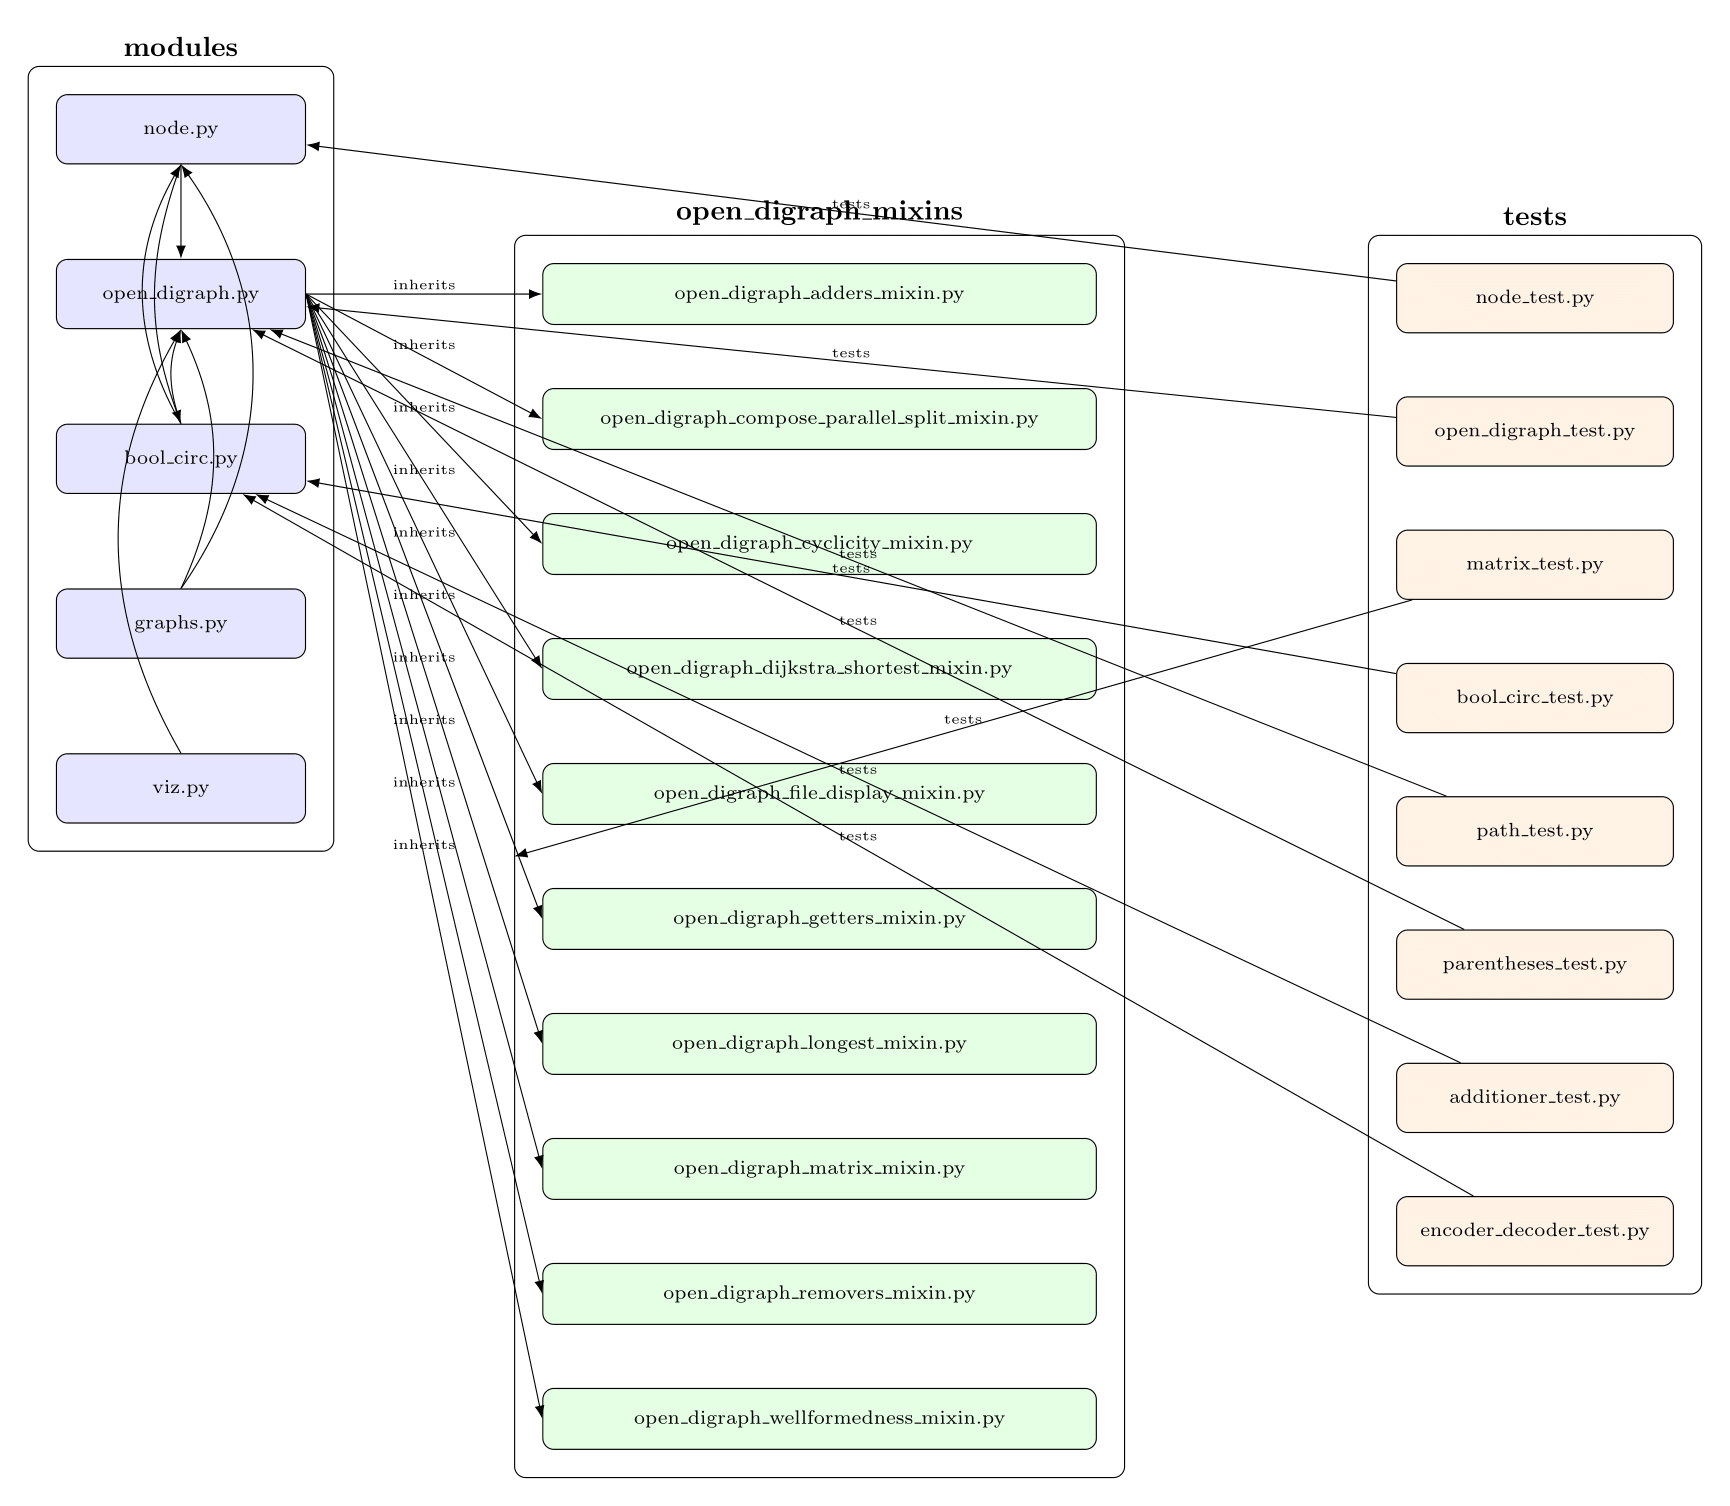
\includegraphics[width=0.8\textwidth]{figures/proj-struct.png}
    \caption{La structure du projet}
\end{figure}
\paragraph{Module \texttt{open\_digraph}.}
\begin{itemize}[nosep]
  \item Structure de base : nœuds et arêtes dirigées.
  \item Système de \emph{mixins} (CRUD, parcours, calcul de distances) pour enrichissement progressif.
\end{itemize}

\paragraph{Extension \texttt{bool\_circ}.}
\begin{itemize}[nosep]
  \item Spécialisation en circuits booléens acycliques avec portes prédéfinies (AND, OR, NOT, XOR...).
  \item Moteur de simplification : associativité, éradication de constantes, fusion de portes.
  \item Évaluateur de signaux binaires.
\end{itemize}

\section{Quelques mots sur le processus de développement du projet}

Le développement de notre projet s'est effectué de manière structurée et
progressive. Nous avons débuté en créant différents types de graphes
aléatoires, notamment des graphes orientés sans cycles, afin d'établir une base
solide avant d'aborder la complexité supérieure des circuits booléens.

Lors du passage aux circuits booléens, nous avons dû résoudre des défis
techniques spécifiques. Parmi ces défis figuraient la gestion des nœuds sans
parents ou sans étiquettes, ainsi que les connexions complexes entre les nœuds.
Pour améliorer la modularité et faciliter l’organisation du code, nous avons
adopté les mixins, ce qui nous a permis une réutilisation efficace du code.

Par la suite, nous avons implémenté une classe spécifique nommée \texttt{bool\_circ},
qui étend notre classe existante open\_digraph. Cette classe est conçue pour
gérer précisément les particularités des circuits booléens, telles que les
portes logiques et les entrées/sorties. Nous avons également mis en place des
méthodes permettant de sauvegarder et visualiser ces circuits via le format
dot, simplifiant ainsi considérablement le processus de débogage et d'analyse
structurelle.

De plus, nous avons développé des algorithmes capables de générer
automatiquement des circuits à partir de formules logiques propositionnelles.
Tout au long du projet, nous avons ajouté de nombreux tests pour garantir la
fiabilité et la robustesse de notre code. Ces tests continus ont permis de
détecter rapidement les erreurs et d'assurer un développement stable. Nous
avons exploré la composition des circuits en parallèle et en séquence, ainsi
que l’analyse des chemins d'information pour optimiser leur fonctionnement.

Nous avons intégré des méthodes d'évaluation des circuits par l'application de
règles de réécriture et développé des techniques pour valider leur exactitude,
en particulier dans le cas de circuits spécifiques comme ceux du code de
Hamming.

Enfin, l'utilisation de \textit{Git} pour le contrôle des versions dès les premières
étapes a été essentielle pour assurer une collaboration efficace et un suivi
précis des différentes évolutions de notre projet.


\section{Analyse de l'additionneur}
Cette section présente une analyse théorique de la profondeur et du nombre de portes logiques dans les circuits additionneurs, construits à partir de cellules adders de 1 bit.

\subsection{1-bit Full Adder}
Une cellule d'additionneur complet de 1 bit prend trois entrées : $a_i$, $b_i$ (les bits à additionner) et $c_i$ (le carry-in). Elle produit deux sorties : $s_i$ (le bit de somme) et $c_{i+1}$ (le carry-out). Les expressions booléennes régissantes sont les suivantes :
\begin{align*}
    s_i &= (a_i \text{\textasciicircum} b_i) \text{\textasciicircum} c_i \\
    c_{i+1} &= (a_i \& b_i) | ((a_i \text{\textasciicircum} b_i) \& c_i)
\end{align*}
Ici, $\text{\textasciicircum}$ indique XOR, $\&$ indique AND, et $|$ indique OR.

\subsubsection{Profondeur logique (niveaux de porte)}
La profondeur logique est le nombre maximal de portes logiques connectées en série entre une entrée primaire (supposée au niveau 0) et une sortie.
\begin{itemize}
    \item \textbf{Sum $s_i$}:
    Le calcul implique deux opérations XOR séquentielles : $x_i = a_i \text{\textasciicircum} b_i$ (1er niveau de porte), suivi de $s_i = x_i \text{\textasciicircum} c_i$ (2ème niveau de porte). La profondeur logique de $s_i$ est de \textbf{2 niveaux de porte}.

    \item \textbf{Carry-out $c_{i+1}$} :
        Le chemin vers $c_{i+1}$ implique :
    \begin{enumerate}
        \item $p_i = a_i \& b_i$ (1er niveau de porte, AND).
        \item $x_i = a_i \text{\textasciicircum} b_i$ (1er niveau de porte, XOR, parallel a $p_i$).
        \item $q_i = x_i \& c_i$ (2ème niveau de la porte, AND, depend de $x_i$).
        \item $c_{i+1} = p_i | q_i$ (3ème niveau de la porte, OR, depend de $p_i$ et $q_i$).
    \end{enumerate}
     La profondeur logique de $c_{i+1}$ est de \textbf{3 niveaux de porte}.
\end{itemize}
La profondeur logique globale de la cellule de l'additionneur complet de 1 bit est déterminée par le chemin le plus long, qui va jusqu'à $c_{i+1}$, soit \textbf{3 niveaux de porte}.
\subsubsection{Nombre de portes logiques}
En supposant que les sous-expressions soient recalculées si elles sont utilisées dans des fonctions de sortie distinctes (par exemple, si les expressions de somme et de report sont analysées indépendamment, comme avec un utilitaire \texttt{parse\_parentheses}) :
\begin{itemize}
    \item For $s_i = (a_i \text{\textasciicircum} b_i) \text{\textasciicircum} c_i$: 2 XOR gates.
    \item For $c_{i+1} = (a_i \& b_i) | ((a_i \text{\textasciicircum} b_i) \& c_i)$: 1 XOR (pour $a_i \text{\textasciicircum} b_i$), 2 portes ET et 1 porte OU (4 portes au total pour la logique de report).
\end{itemize}
Le nombre total de portes logiques est de $2 + 4 = \textbf{6}$.

\subsection{Additionneur simple de $M$ bits}
Un additionneur simple de $M$ bits est formé par la mise en cascade de $M$ cellules de l'additionneur complet de 1 bit. La sortie $c_{i+1}$ de l'étage $i$ devient l'entrée de l'étage $i+1$. La retenue initiale, $c_0$, est généralement égale à  '0'.

\subsubsection{Profondeur logique (niveaux de porte)}
Le chemin critique qui détermine la profondeur est la propagation de la retenue du LSB(Least significant bit) au MSB(Most significant bit).
\begin{itemize}
    \item Stage 0 (LSB): Produces $c_1$ at a depth of 3 gate levels.
    \item Subsequent stages $i > 0$: The logic to produce $c_{i+1}$ from $c_i$ adds 2 gate levels to the path of $c_i$. Thus, $depth(c_{i+1}) = depth(c_i) + 2$.
    \item Tracing carry depths: $depth(c_1) = 3$; $depth(c_k) = 3 + (k-1) \times 2 = 2k + 1$.
    \item The final carry-out $c_M$ has $depth(c_M) = 2M + 1$.
    \item The MSB sum $s_{M-1}$ depends on $c_{M-1}$ (depth $2(M-1)+1$) and requires 2 more XOR levels, resulting in $depth(s_{M-1}) = (2(M-1)+1) + 2 = 2M+1$.
\end{itemize}
La profondeur logique d'un additionneur de $M$ bits est $\boldsymbol{D(M) = 2M + 1}$.\\
Par exemple :
\begin{enumerate}
    \item $M=1 \Rightarrow Profondeur=3$; 
    \item $M=2 \Rightarrow Profondeur=5$;
    \item $M=4 \Rightarrow Profondeur=9$.
\end{enumerate}


\subsubsection{Chemin le plus court (niveaux de porte)}
Le chemin logique le plus court est généralement celui de la somme LSB $s_0 = (a_0 \text{\textasciicircum} b_0) \text{\textasciicircum} c_0$. Cela implique \textbf{2 niveaux de porte} (deux XOR).

\subsection{Influence de la duplication des signaux sur la profondeur du graphe structurel}
Dans les représentations graphiques des circuits, les signaux (sorties de portes ou entrées primaires) servent souvent d'entrées à plusieurs portes ultérieures (split-out). Pour gérer cette situation, les structures des graphes comprennent des "nœuds de copie" (nœuds avec une étiquette vide \texttt{""}), qui dupliquent ou traversent les signaux.

L'introduction de ces nœuds de copie ajoute des couches structurelles au graphe. Alors que la profondeur logique ne prend en compte que la cascade de portes opérationnelles (AND, OR, XOR), la profondeur structurelle mesurée sur le graphe peut être plus importante. Chaque cas où un signal (par exemple, $a_i$, $b_i$, $c_i$) est acheminé vers plusieurs portes opérationnelles distinctes peut nécessiter une couche intermédiaire de nœuds de copie. Par conséquent, la profondeur structurelle globale du graphe, reflétant toutes ces couches opérationnelles et d'acheminement des signaux, peut dépasser la profondeur de la porte purement opérationnelle. Par exemple, pour un additionneur complet de 1 bit, la profondeur augmente de 2.

\begin{figure}[H]
    \centering
    \begin{minipage}{0.49\textwidth}
        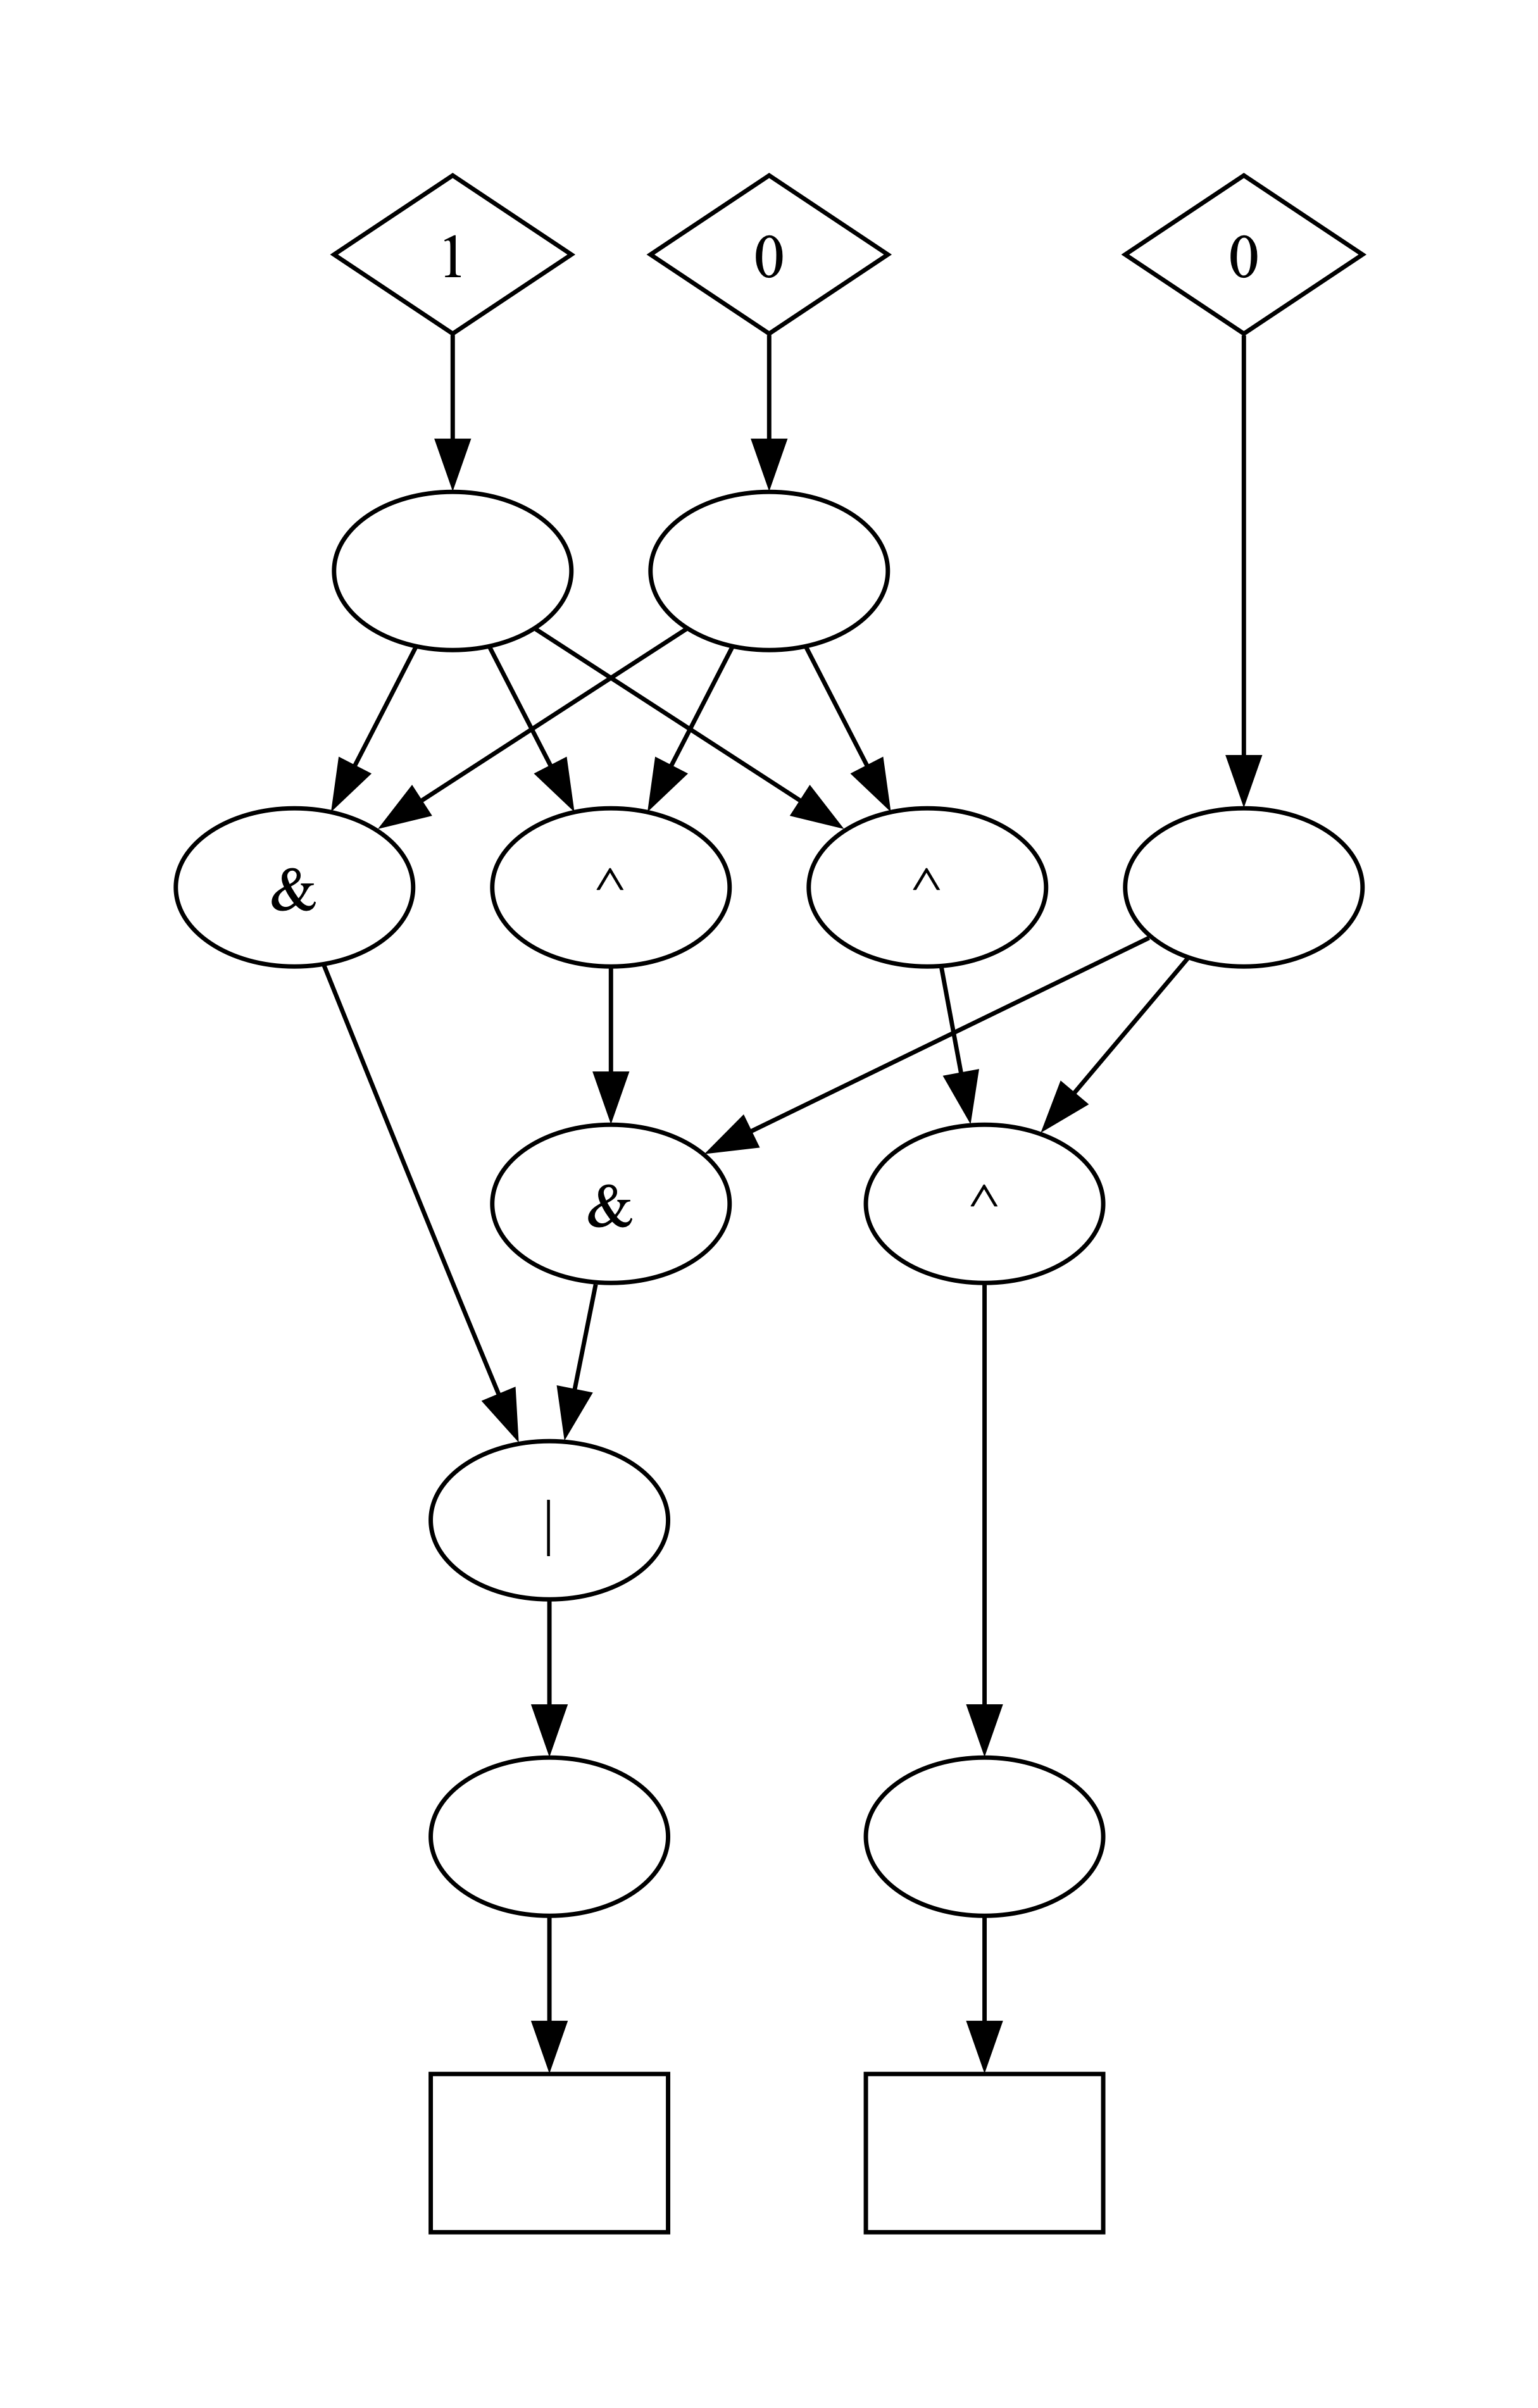
\includegraphics[width=0.8\textwidth]{figures/adder_1_bit.png}
    \end{minipage}
    \begin{minipage}{0.49\textwidth}
        \includegraphics[width=0.8\textwidth]{figures/adder_3_bit.png}
    \end{minipage}
    \caption{Exemples des adders des registres $2^0$ et  $2^1$ réspéctivement}
    \label{fig:}
\end{figure}

\section{Carry-Lookahead Adders}

L'additionneur de retenue (CLA) réduit la profondeur de calcul en pré-calculant les signaux de "propagation" ($P_i$) et de "génération" ($G_i$) pour chaque bit $i$ : $P_i = a_i \text{\textasciicircum} b_i$ et $G_i = a_i \& b_i$. Cela permet de déterminer les reports de manière plus directe. L'implémentation discutée utilise des blocs CLA de 4 bits, qui sont ensuite enchaînés pour des additionneurs plus grands de $4N$ bits.
\subsection{Analyse du bloc Carry-Lookahead 4 bits}
Un bloc de 4 bits traite les entrées $a_i, b_i$ (pour $i \in [0,3]$) et un \textit{carry-in} de bloc $C_{in_0}$, produisant les sommes $S_i$ et un \textit{carry-out} de bloc $C_{out_3}$ (également $C_4$).

\subsubsection{Génération des signaux P et G (bloc de 4 bits)}
\begin{itemize}
    \item \textbf{Nombre de portes :} 4 XORs (for $P_0..P_3$) + 4 ANDs (for $G_0..G_3$) = \textbf{8 portes}.
    \item \textbf{Profondeur logique :} Tous les $P_i, G_i$ sont calculés en parallèle : \textbf{1 niveau de porte}.
\end{itemize}

\subsubsection{Calcul de retenue (itératif dans un bloc de 4 bits)}
On utilise $C_{out,i} = G_i | (P_i \& C_{in,i})$, où $C_{in,i+1} = C_{out,i}$.
\begin{itemize}
    \item \textbf{Nombre de portes:} Pour 4 étapes ($C_{out,0}$ a $C_{out,3}$): $4 \times (1 \text{ AND} + 1 \text{ OR}) = \textbf{8 portes}$.
    \item \textbf{Profondeur logique :}
        
        $P_i, G_i$ sont à la profondeur 1. $C_{in,0}$ est à la profondeur 0.
        \begin{enumerate}
           
        \item $depth(C_{out,0})=3$ 
        \item $depth(C_{out,1})=5$
        \item $depth(C_{out,2})=7$
        \item $depth(C_{out,3})=9$.
        \end{enumerate}
        
   Le report de bloc $C_{out,3}$ est à \textbf{9 niveaux de porte}.
\end{itemize}

\subsubsection{Calcul de la somme (bloc de 4 bits))}
La somme des bits est calculée à l'aide de la formule $S_i = P_i \text{\textasciicircum} C_i$. La profondeur de chaque $S_i$ dépend des temps d'arrivée (profondeurs) de $P_i$ et $C_i$. Nous rappelons que tous les signaux $P_i$ sont disponibles à la profondeur 1, et que les porteuses $C_i$ (entrées de l'étage $i$) sont disponibles à des profondeurs variables : $C_0$ à la profondeur 0, $C_1$ à la profondeur 3, $C_2$ à la profondeur 5, et $C_3$ à la profondeur 7. La porte XOR pour $S_i$ ajoute un niveau à la profondeur maximale de ses entrées.

\begin{itemize}
    \item Pour $S_0 = P_0 \text{\textasciicircum} C_0$:
        $depth(S_0) = \max(depth(P_0), depth(C_0)) + 1 = \max(1, 0) + 1 = \textbf{2}$.
    \item Pour $S_1 = P_1 \text{\textasciicircum} C_1$:
        $depth(S_1) = \max(depth(P_1), depth(C_1)) + 1 = \max(1, 3) + 1 = \textbf{4}$.
    \item Pour $S_2 = P_2 \text{\textasciicircum} C_2$:
        $depth(S_2) = \max(depth(P_2), depth(C_2)) + 1 = \max(1, 5) + 1 = \textbf{6}$.
    \item Pour $S_3 = P_3 \text{\textasciicircum} C_3$:
        $depth(S_3) = \max(depth(P_3), depth(C_3)) + 1 = \max(1, 7) + 1 = \textbf{8}$.
\end{itemize}
La profondeur logique maximale parmi les sorties de la somme est pour $S_3$, qui est de \textbf{8 niveaux de porte}.

\subsubsection{Totaux pour un bloc CLA de 4 bits}
\begin{itemize}
    \item \textbf{Nombre total de portes logiques:} 8 (P/G) + 8 (Carry) + 4 (Sums) = \textbf{20 portes}.
    \item \textbf{Profondeur logique globale:} La profondeur déterminée est de \textbf{9 niveaux de porte} car pour la retenue, nous avons besoin de 9 niveaux de porte.
\end{itemize}


\subsubsection{Chemin le plus court (niveaux de porte)}
Il reste $S_0$ dans le premier bloc (LSB) : $\boldsymbol{2}$ niveaux de porte.

\subsection{Influence de la duplication des signaux sur la profondeur du graphe structurel (CLA)}
La construction directe de blocs CLA de 4 bits implique souvent des "nœuds de copie" comme dans l'additionneur simple. Ces nœuds non opérationnels augmentent la profondeur structurelle du graphe. Par exemple, un seul bloc CLA de 4 bits avec une profondeur logique de 9 peut présenter une profondeur structurelle de graphe plus élevée (15 lorsque l'on calcule la profondeur en utilisant le tri topologique du graphe).

\begin{figure}[H]
    \centering
    \includegraphics[width=0.8\textwidth]{figures/carry_lookahead_4.png}
    \caption{Exemple d'un carry look ahead}
    \label{fig:}
\end{figure}




\section{Évaluation d'un demi-additionneur (Half Adder)}\label{sec:halfadder}
Nous illustrons le mécanisme interne du module \texttt{bool\_circ} en évaluant un demi-additionneur appliqué à deux entiers codés sur 4 bits (par exemple 2 et 3).

\subsection{Création du graphe initial}
\begin{enumerate}[label=\arabic*.,nosep]
  \item \textbf{Génération des circuits booléens.} Chaque entier est converti en un sous-graphe de largeur 4, chaque bit devenant un nœud d'entrée.
  \item \textbf{Construction du half adder.} Pour chaque position de bit, les deux nœuds d'entrée se connectent à un sous-graphe implémentant une porte \texttt{XOR} (somme partielle) et une porte \texttt{AND} (retenue).
  \item Assemblage en un graphe complet du demi-additionneur.
\end{enumerate}

\subsection{Évaluation et simplification itérative du graphe}
\begin{enumerate}[label=\arabic*.,nosep]
  \item \textbf{Initialisation.} Graphe complet issu de l'assemblage.
  \item \textbf{Passes de simplification.} À chaque passe, pour chaque nœud, on teste et applique localement la première règle de simplification disponible. On répète jusqu'au point fixe (aucune règle applicable).
\end{enumerate}

\subsection{Règles de simplification}

Lors de chaque passe de l’algorithme \texttt{evaluate()}, on parcourt tous les nœuds du graphe et on applique localement l’une des règles ci-dessous dès qu’elle est applicable. On répète les passes tant qu’au moins une règle peut encore s’appliquer.

\subsubsection{Propagation et élimination de constantes}

\begin{description}
    \item[Copie de constante (\texttt{constant\_copy\_transform})]
    Si une porte de copie (\texttt{""}) reçoit en entrée une constante (\texttt{0} ou \texttt{1}), on la remplace par autant de constantes fraîches qu’il y a de sorties, puis on supprime la porte de copie et éventuellement la constante d’origine si elle devient isolée.

    \item[Inversion de constante (\texttt{constant\_not\_transform})]
    Si une porte NOT (\texttt{\textasciitilde}) a pour unique parent une constante, on la remplace par la constante inversée directement connectée à la sortie, et on supprime la porte NOT (et éventuellement la constante source si elle devient isolée).
\end{description}

\subsubsection{Simplifications logiques basées sur AND/OR/XOR}

\begin{description}
    \item[AND-0 (\texttt{transform\_and\_zero})]
    Si un AND (\texttt{\&}) a un parent \texttt{0}, le résultat est \texttt{0} : on reconnecte \texttt{0} à la sortie, on remplace chaque autre entrée par sa propre porte de copie, puis on supprime l’AND.

    \item[AND-1 (\texttt{transform\_and\_one})]
    Si un AND a un parent \texttt{1}, cette entrée est neutre : on supprime simplement tous les fils issus de ce \texttt{1} vers l’AND, puis on supprime le \texttt{1} isolé.

    \item[OR-0 (\texttt{transform\_or\_zero})]
    Si un OR (\texttt{|}) a un parent \texttt{0}, cette entrée est neutre : on supprime tous les fils de ce \texttt{0} vers l’OR, puis on supprime le \texttt{0} isolé.

    \item[OR-1 (\texttt{transform\_or\_one})]
    Si un OR a un parent \texttt{1}, le résultat est \texttt{1} : on reconnecte ce \texttt{1} à la sortie, on remplace chaque autre entrée par sa propre copie, puis on supprime l’OR.

    \item[XOR-0 (\texttt{transform\_xor\_zero})]
    Dans un XOR (\texttt{\^}), un \texttt{0} en entrée est neutre : on supprime simplement ses fils vers le XOR, et on supprime le \texttt{0} isolé.

    \item[XOR-1 (\texttt{transform\_xor\_one})]
    Un \texttt{1} dans un XOR équivaut à une inversion : on enlève l’arête \texttt{1}$\rightarrow$XOR, on place un NOT à la sortie du XOR et on supprime le \texttt{1} isolé.

    \item[Porte sans entrée]
    \begin{itemize}
        \item \texttt{OR}/\texttt{XOR} vide $\rightarrow$ \texttt{0} (\texttt{transform\_in\_zero})
        \item \texttt{AND} vide $\rightarrow$ \texttt{1} (\texttt{transform\_in\_one})
    \end{itemize}
    Si une porte logique n’a plus d’entrées, on la remplace par la constante neutre appropriée, reconnectée à ses enfants.
\end{description}

\subsubsection{Règles d’associativité et d’involution}

\begin{description}
    \item[Associativité du XOR (\texttt{transform\_associative\_xor})]
    Deux XOR consécutifs sont fusionnés en un seul XOR dont les parents sont la réunion de leurs anciennes entrées.

    \item[Fusion de copies (\texttt{transform\_associative\_copy})]
    Deux portes de copie successives sont fusionnées en une seule.

    \item[Involution du XOR (\texttt{transform\_involution\_xor})]
    Si deux copies identiques se reroutent vers un même XOR avec une multiplicité paire, on supprime les deux (effet neutre), sinon on laisse une connexion unique.

    \item[Double négation (\texttt{transform\_not\_involution})]
    Deux NOT en série (\texttt{\textasciitilde\textasciitilde}) s’annulent : on raccorde directement l’entrée à la sortie et on supprime les deux portes NOT.
\end{description}

\subsubsection{Gestion des portes mortes et déplacement de NOT}

\begin{description}
    \item[Effacement d’opérateur isolé (\texttt{transform\_erase\_operator})]
    Une porte de copie sans sortie (mais avec un parent) est supprimée, et on reconnecte ses anciens entrées directement à de nouvelles copies si nécessaire.

    \item[Sortie du NOT hors du XOR (\texttt{transform\_xor\_if\_has\_parent\_not})]
    Si un XOR a un parent NOT, on déplace ce NOT en aval du XOR (équivalence de \texttt{\textasciitilde}(a$\oplus$b) = a$\oplus$b puis \texttt{NOT}).

    \item[Sortie du NOT hors de la copie (\texttt{transform\_copy\_if\_has\_parent\_not})]
    Si une copie a un parent NOT, on récupère le signal original avant NOT, on fuse et on refait les NOT nécessaires en aval.
\end{description}

\subsubsection{Répétition jusqu’au point fixe}
\begin{itemize}
    \item On recommence autant de passes que nécessaire, tant qu’au moins une règle a été appliquée lors de la passe précédente.
    \item Le processus se termine lorsque plus aucune simplification n’est possible (atteinte d’un point fixe).
\end{itemize}

\subsection{Résultat final}
Le graphe maximalement réduit fournit les valeurs de Somme (S) et Retenue (C). Pour notre exemple (2 + 3), 62 passes d'évaluation ont été nécessaires.

La visualisation d'évaluation de \textit{half-adder} est disponible à la fin du rapport (voir les figures \ref{fig:half-adder-apres-initialisation}, \ref{fig:half-adder-apres-le-premier-pas-devaluate}, \ref{fig:half-adder-comparaison}, \ref{fig:etapes-avant-la-finalisation-de-l-evaluation-de-half-adder}, \ref{fig:etat-de-half-adder-apres-l-evaluation-complete})

\section{Vérification de la propriété principale du code de Hamming}
Pour valider que l'encodeur et le décodeur se composent en l'identité (correction d'une erreur simple), nous suivons :

\subsection{Approche générale}

Pour valider que l’encodeur et le décodeur se composent en l’identité (et que l’on corrige toute erreur simple, mais pas toute double erreur), nous suivons quatre grandes étapes~:

\begin{enumerate}
    \item \textbf{Génération des graphes}
    \begin{itemize}
        \item \textbf{Encodeur 4 bits~:} à partir d’un mot de 4 bits, on construit le graphe d’encodage. Chaque bit de donnée est relié à des portes de parité (XOR) qui produisent les trois bits de contrôle.
        \item \textbf{Décodeur 4 bits~:} on élabore un graphe de décodage composé de modules de syndrome (XOR et AND) et d’un réseau de correction (portes conditionnelles) capable de détecter et corriger une seule erreur.
    \end{itemize}

    \item \textbf{Composition des graphes}
    \begin{itemize}
        \item On relie les sorties de l’encodeur aux entrées du décodeur pour obtenir un seul graphe «~encodeur$\rightarrow$décodeur~».
        \item Cette étape est automatique~: la méthode de composition s’appuie sur les listes d’identifiants de nœuds de sortie et d’entrée pour tisser les connexions appropriées.
    \end{itemize}

    \item \textbf{Simplification (évaluation)}
    \begin{itemize}
        \item Appel de la méthode \texttt{evaluate()} sur le graphe composé~:
        \begin{itemize}
            \item Chaque passe balaie tous les nœuds à la recherche de motifs simplifiables (fusion de portes identiques, élimination de constantes, propagation de NOT).
            \item Dès qu’une transformation s’applique, le graphe est modifié et une nouvelle passe recommence.
            \item Le processus s’arrête au point fixe, c’est-à-dire lorsqu’aucune règle n’est plus applicable.
        \end{itemize}
    \end{itemize}

    \item \textbf{Extraction et comparaison des résultats}
    \begin{itemize}
        \item On lit les quatre bits de sortie restants et on forme un mot binaire.
        \item On compare ce mot au mot d’entrée d’origine, pour chacun des scénarios de test.
    \end{itemize}
\end{enumerate}

\subsection{Cas de test}

\subsubsection*{Sans erreur}
\begin{itemize}
    \item Composition de l’encodeur et du décodeur sur le mot initial (voir les figures de l'encodeur: \ref{fig:encoder-no-error}, le décodeur: \ref{fig:decoder-no-error}, et la composition des deux dernièrs: \ref{fig:compos-enc-dec-no-error})
    \item Après évaluation, le graphe final se réduit à quatre fils directs (identité). (voir la figure: \ref{fig:enc-dec-identity})
    \item Résultat~: mot de sortie = mot d’entrée.
\end{itemize}

    
    
\subsubsection*{Une erreur unique}
\begin{itemize}
    \item Injection d’une inversion sur l’un des quatre bits en sortie de l’encodeur. (voir les figures du décodeur: \ref{fig:decoder-with-one-error} et de la composition: \ref{fig:encode-decode-compose-one-error}) 
    \item Le décodeur calcule un syndrome, active la porte de correction correspondante, puis le graphe se simplifie en identité. (voir la figure: \ref{fig:enc-dec-identity})
    \item Résultat~: même mot restauré, quelle que soit la position de l’erreur.
\end{itemize}

\subsubsection*{Deux erreurs}
\begin{itemize}
    \item Inversions sur deux positions distinctes. (voir le décodeur: figure \ref{fig:decoder-two-errors})
    \item Le graphe final, simplifié au maximum, reste différent de l’identité, et le mot en sortie ne correspond plus à l’entrée. (voir l'identité avec erreur: figure \ref{fig:identity-two-errors})
\end{itemize}

\subsubsection*{Exemples des tests en python}
\begin{lstlisting}[caption={tests}, label={lst:tests-de-encodeur}]
def test_enc_dec_compose_eval_gives_identity(self):
    # define the sequence of bits to encode
    bit1, bit2, bit3, bit4 = '0', '1', '0', '1'
    res = bit1+bit2+bit3+bit4

    # construct encoder
    enc_g = bool_circ.generate_4bit_encoder(bit1, bit2, bit3, bit4)
    # construct decoder
    dec_g = bool_circ.generate_4bit_decoder('', '', '', '', '', '', '')
    # compose both
    comp = dec_g.compose(enc_g)
    comp = bool_circ(comp)
    # evaluate to get the result
    comp.evaluate()

    # verify that we obtain an identity graph
    self.assertEqual(len(comp.get_nodes_ids()), 4*2) 

    # compare the evaluated result
    self.assertEqual(get_result_of_evaluated_enc_dec(comp), res)

def test_enc_dec_compose_eval_gives_identity_with_changed_bit_1(self):
    bit1, bit2, bit3, bit4 = '0', '1', '0', '1'
    res = bit1+bit2+bit3+bit4

    enc_g = bool_circ.generate_4bit_encoder(bit1, bit2, bit3, bit4)
    # ajoute d'une porte non
    dec_g = bool_circ.generate_4bit_decoder('~', '', '', '', '', '', '')
    comp = dec_g.compose(enc_g)
    comp = bool_circ(comp)
    comp.evaluate()

    self.assertEqual(len(comp.get_nodes_ids()), 4*2) 

    self.assertEqual(get_result_of_evaluated_enc_dec(comp), res)

def test_enc_dec_compose_eval_gives_identity_with_changed_bit_2(self):
    bit1, bit2, bit3, bit4 = '0', '1', '0', '1'
    res = bit1+bit2+bit3+bit4

    enc_g = bool_circ.generate_4bit_encoder(bit1, bit2, bit3, bit4)
    # ajoute d'une porte non pour l'autre bit
    dec_g = bool_circ.generate_4bit_decoder('', '', '', '~', '', '', '')
    comp = dec_g.compose(enc_g)
    comp = bool_circ(comp)
    comp.evaluate()

    self.assertEqual(len(comp.get_nodes_ids()), 4*2) 

    self.assertEqual(get_result_of_evaluated_enc_dec(comp), res)

def test_enc_dec_compose_eval_with_2bits_changed(self):
    bit1, bit2, bit3, bit4 = '0', '1', '0', '1'
    res = bit1+bit2+bit3+bit4

    enc_g = bool_circ.generate_4bit_encoder(bit1, bit2, bit3, bit4)
    # ajoute de deux portes non
    dec_g = bool_circ.generate_4bit_decoder('', '', '', '~', '', '', '~')
    comp = dec_g.compose(enc_g)
    comp = bool_circ(comp)
    comp.evaluate()

    self.assertEqual(len(comp.get_nodes_ids()), 4*2) 

    self.assertNotEqual(get_result_of_evaluated_enc_dec(comp), res)
\end{lstlisting}

\section{Visualisation des étapes intermidiaires}
\subsection{Les figures de l'additionneur}
\begin{figure}[H]
    \centering
    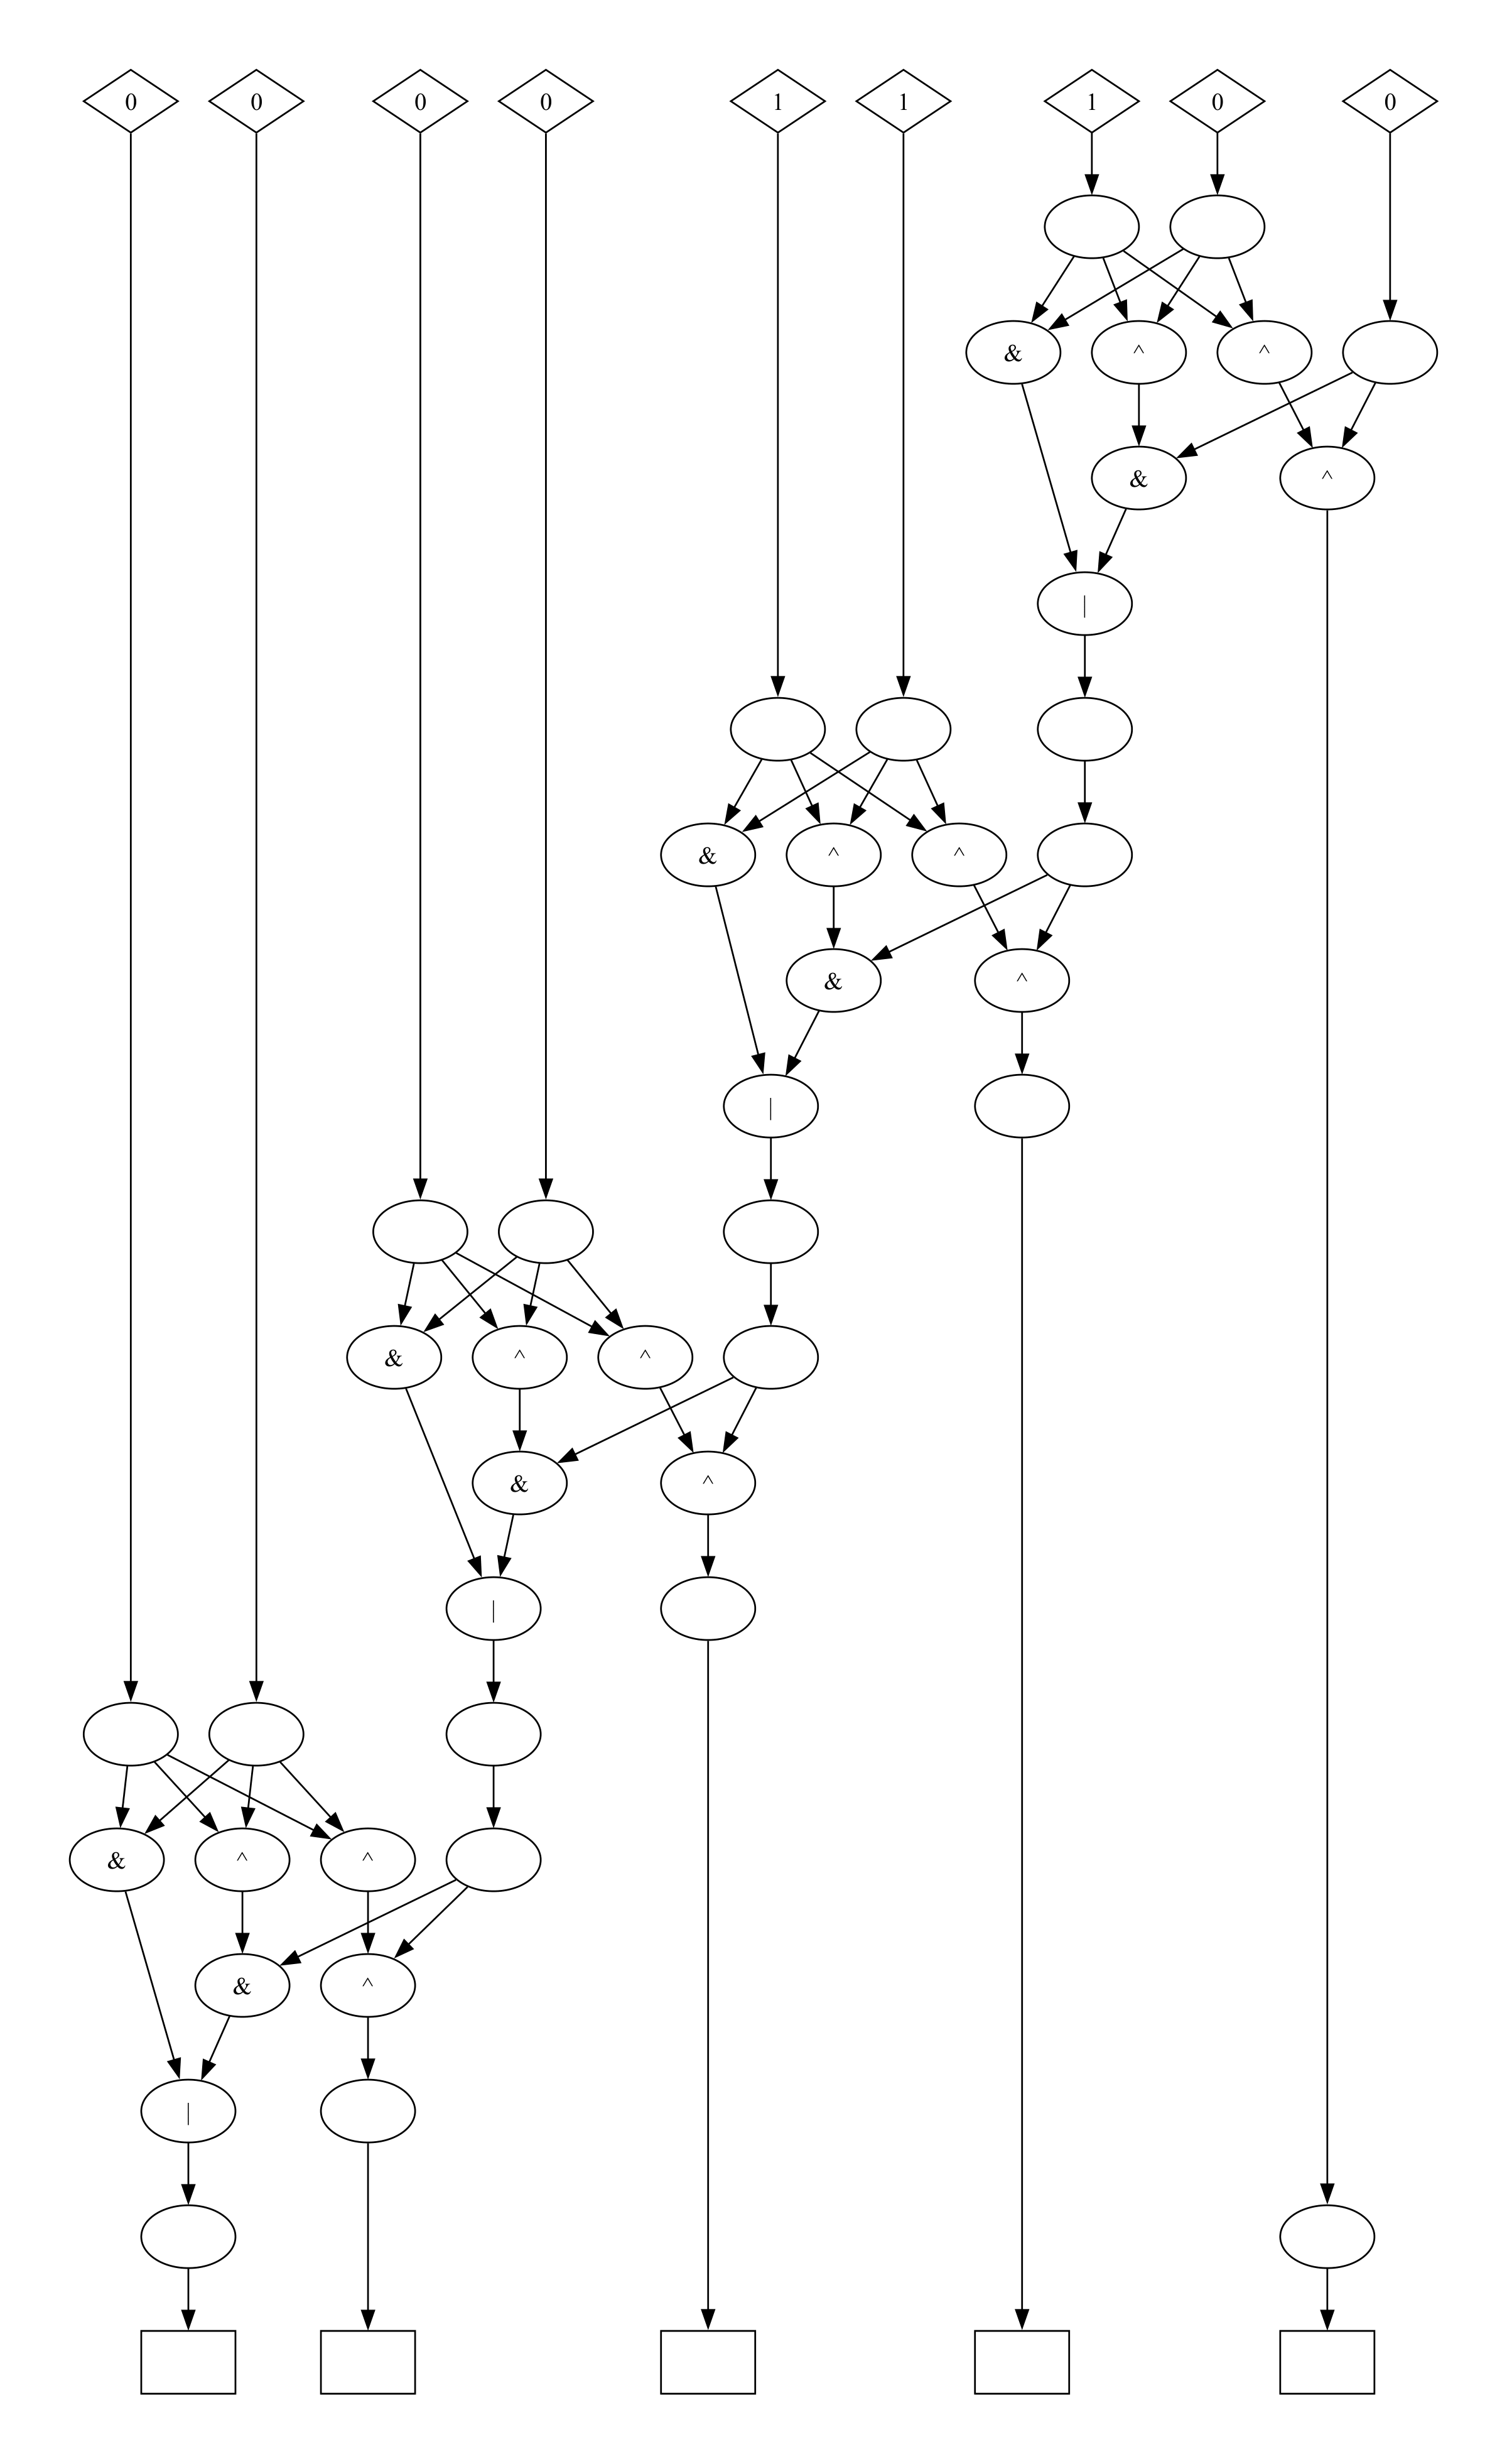
\includegraphics[width=0.8\textwidth]{figures/half_adder/adder_1-1.png}
    \caption{Half-adder juste après l'initialisation}
    \label{fig:half-adder-apres-initialisation}
\end{figure}
\begin{figure}[H]
    \centering
    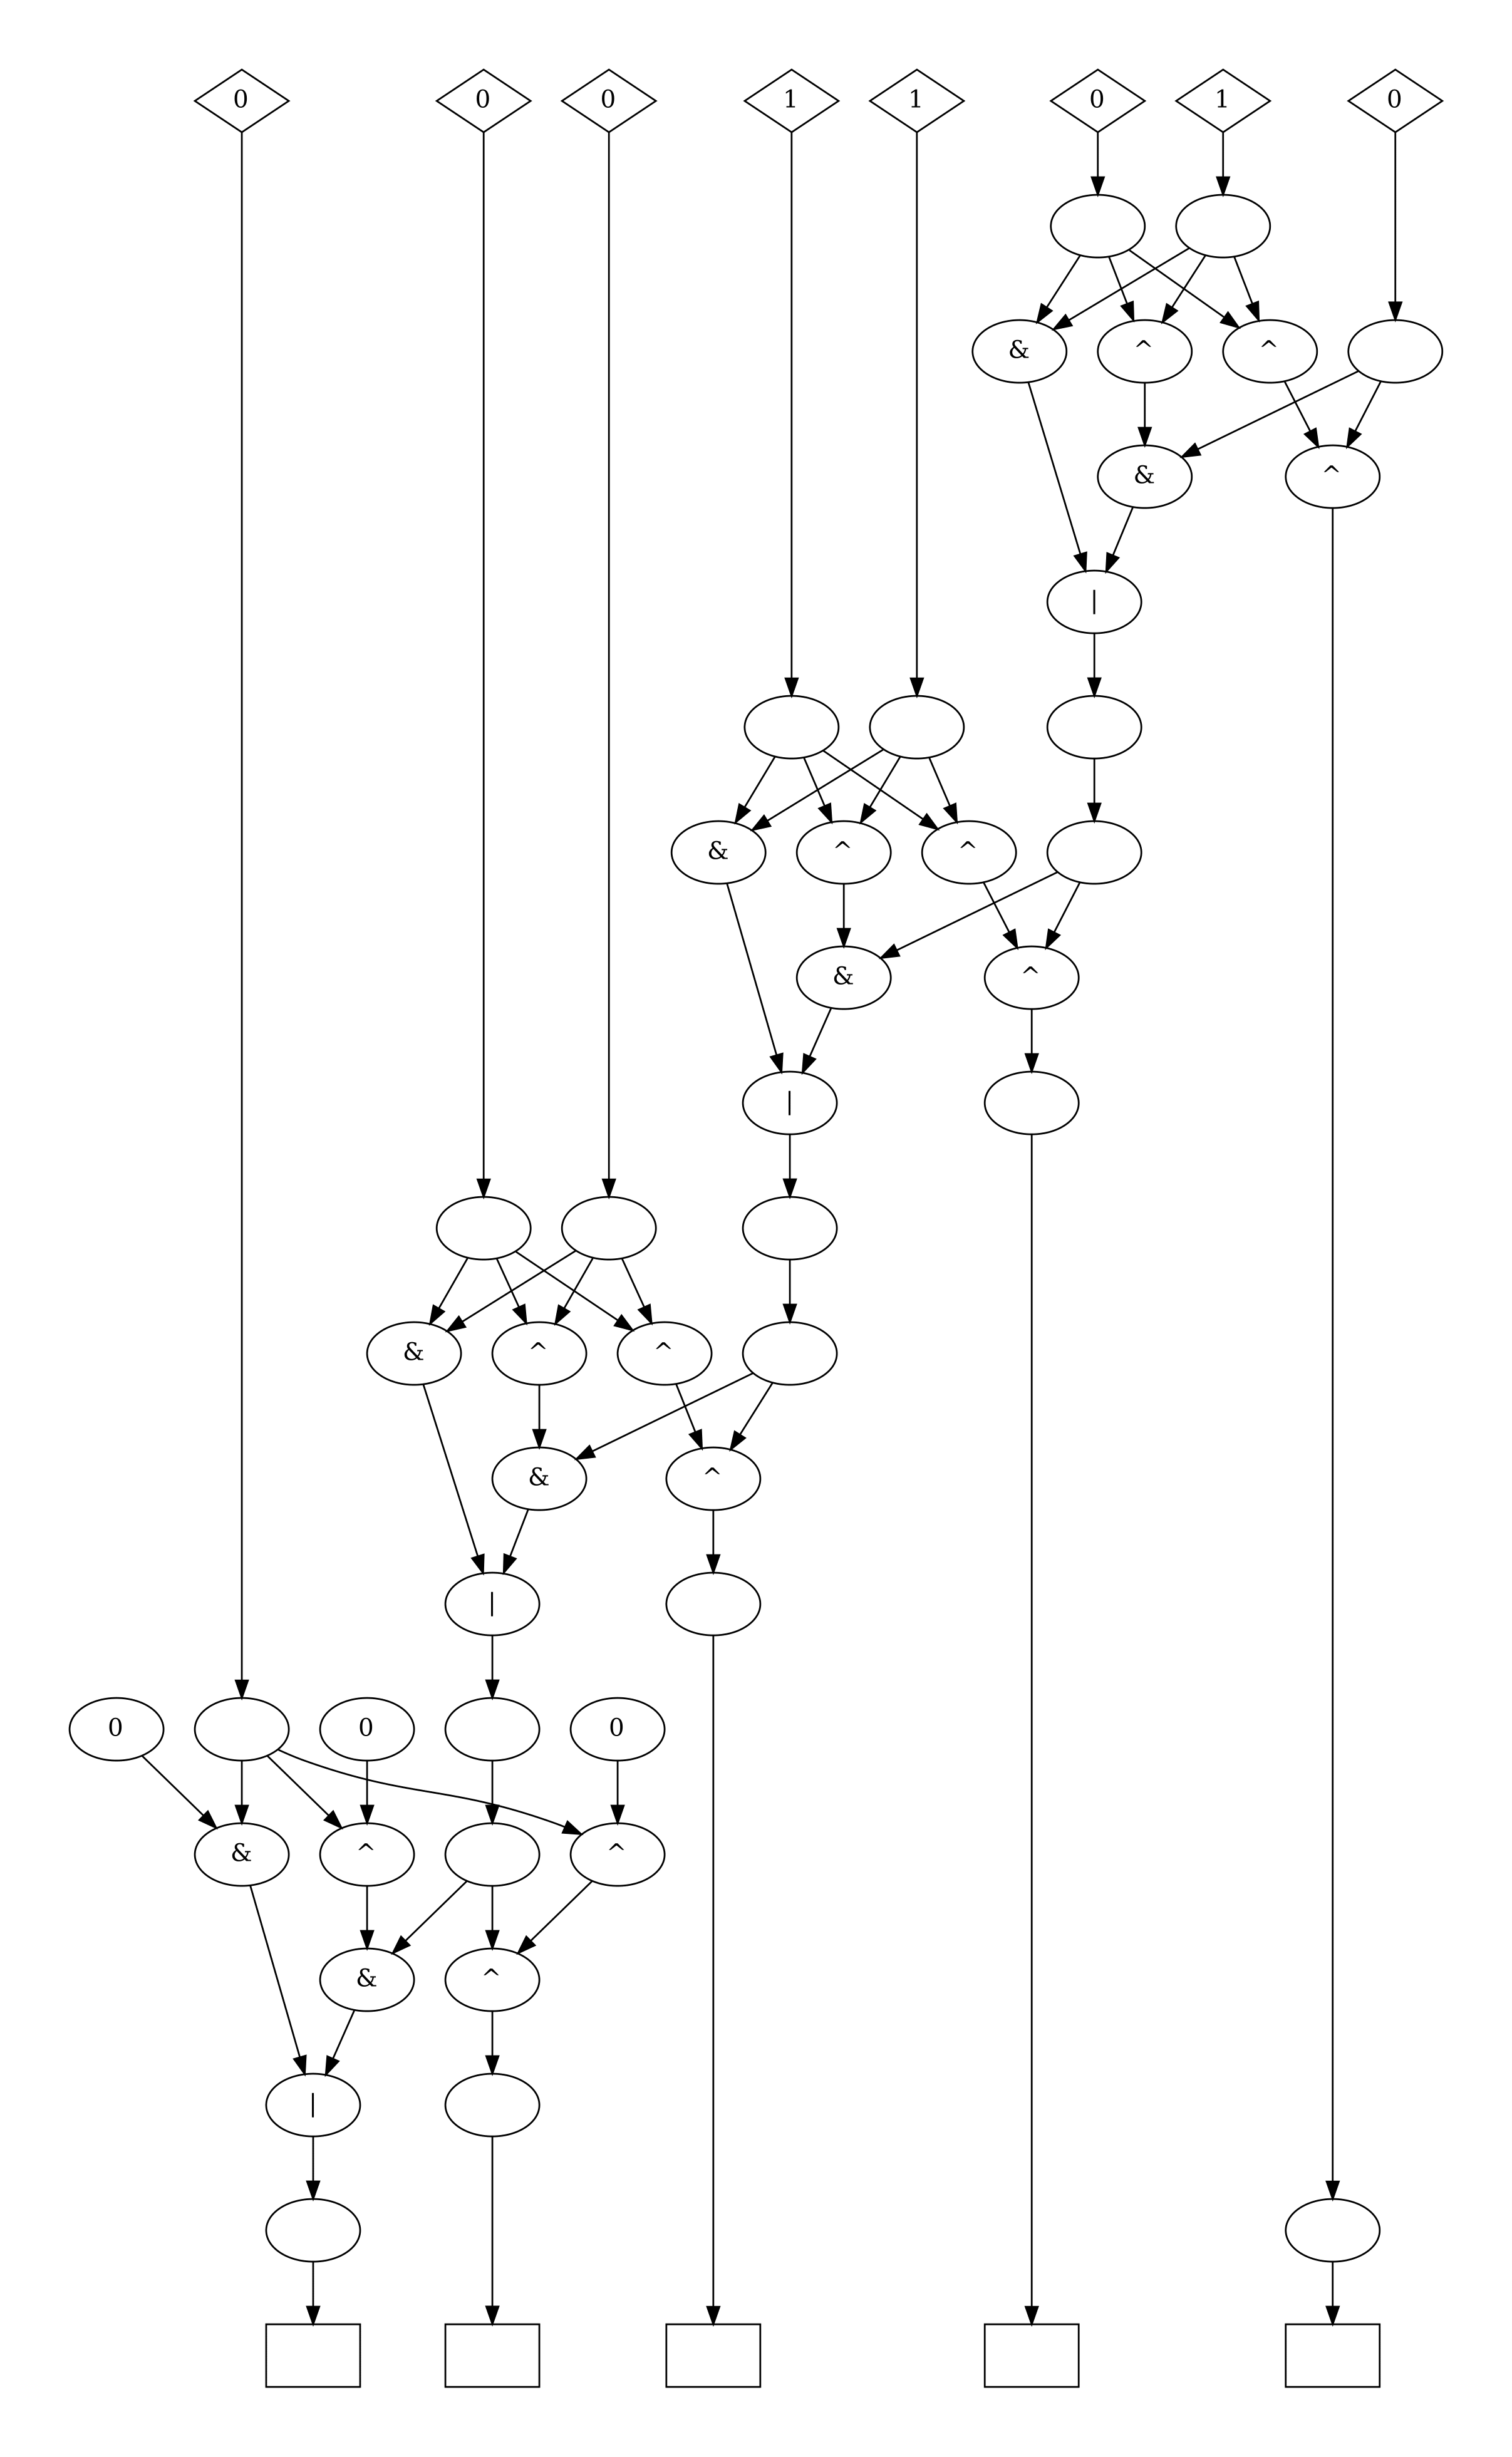
\includegraphics[width=0.8\textwidth]{figures/half_adder/debug_evualte_0-1.png}
    \caption{Half-adder après le premier pas d'evaluate}
    \label{fig:half-adder-apres-le-premier-pas-devaluate}
\end{figure}
\begin{figure}[H]
    \centering
        \begin{minipage}{0.49\textwidth}
            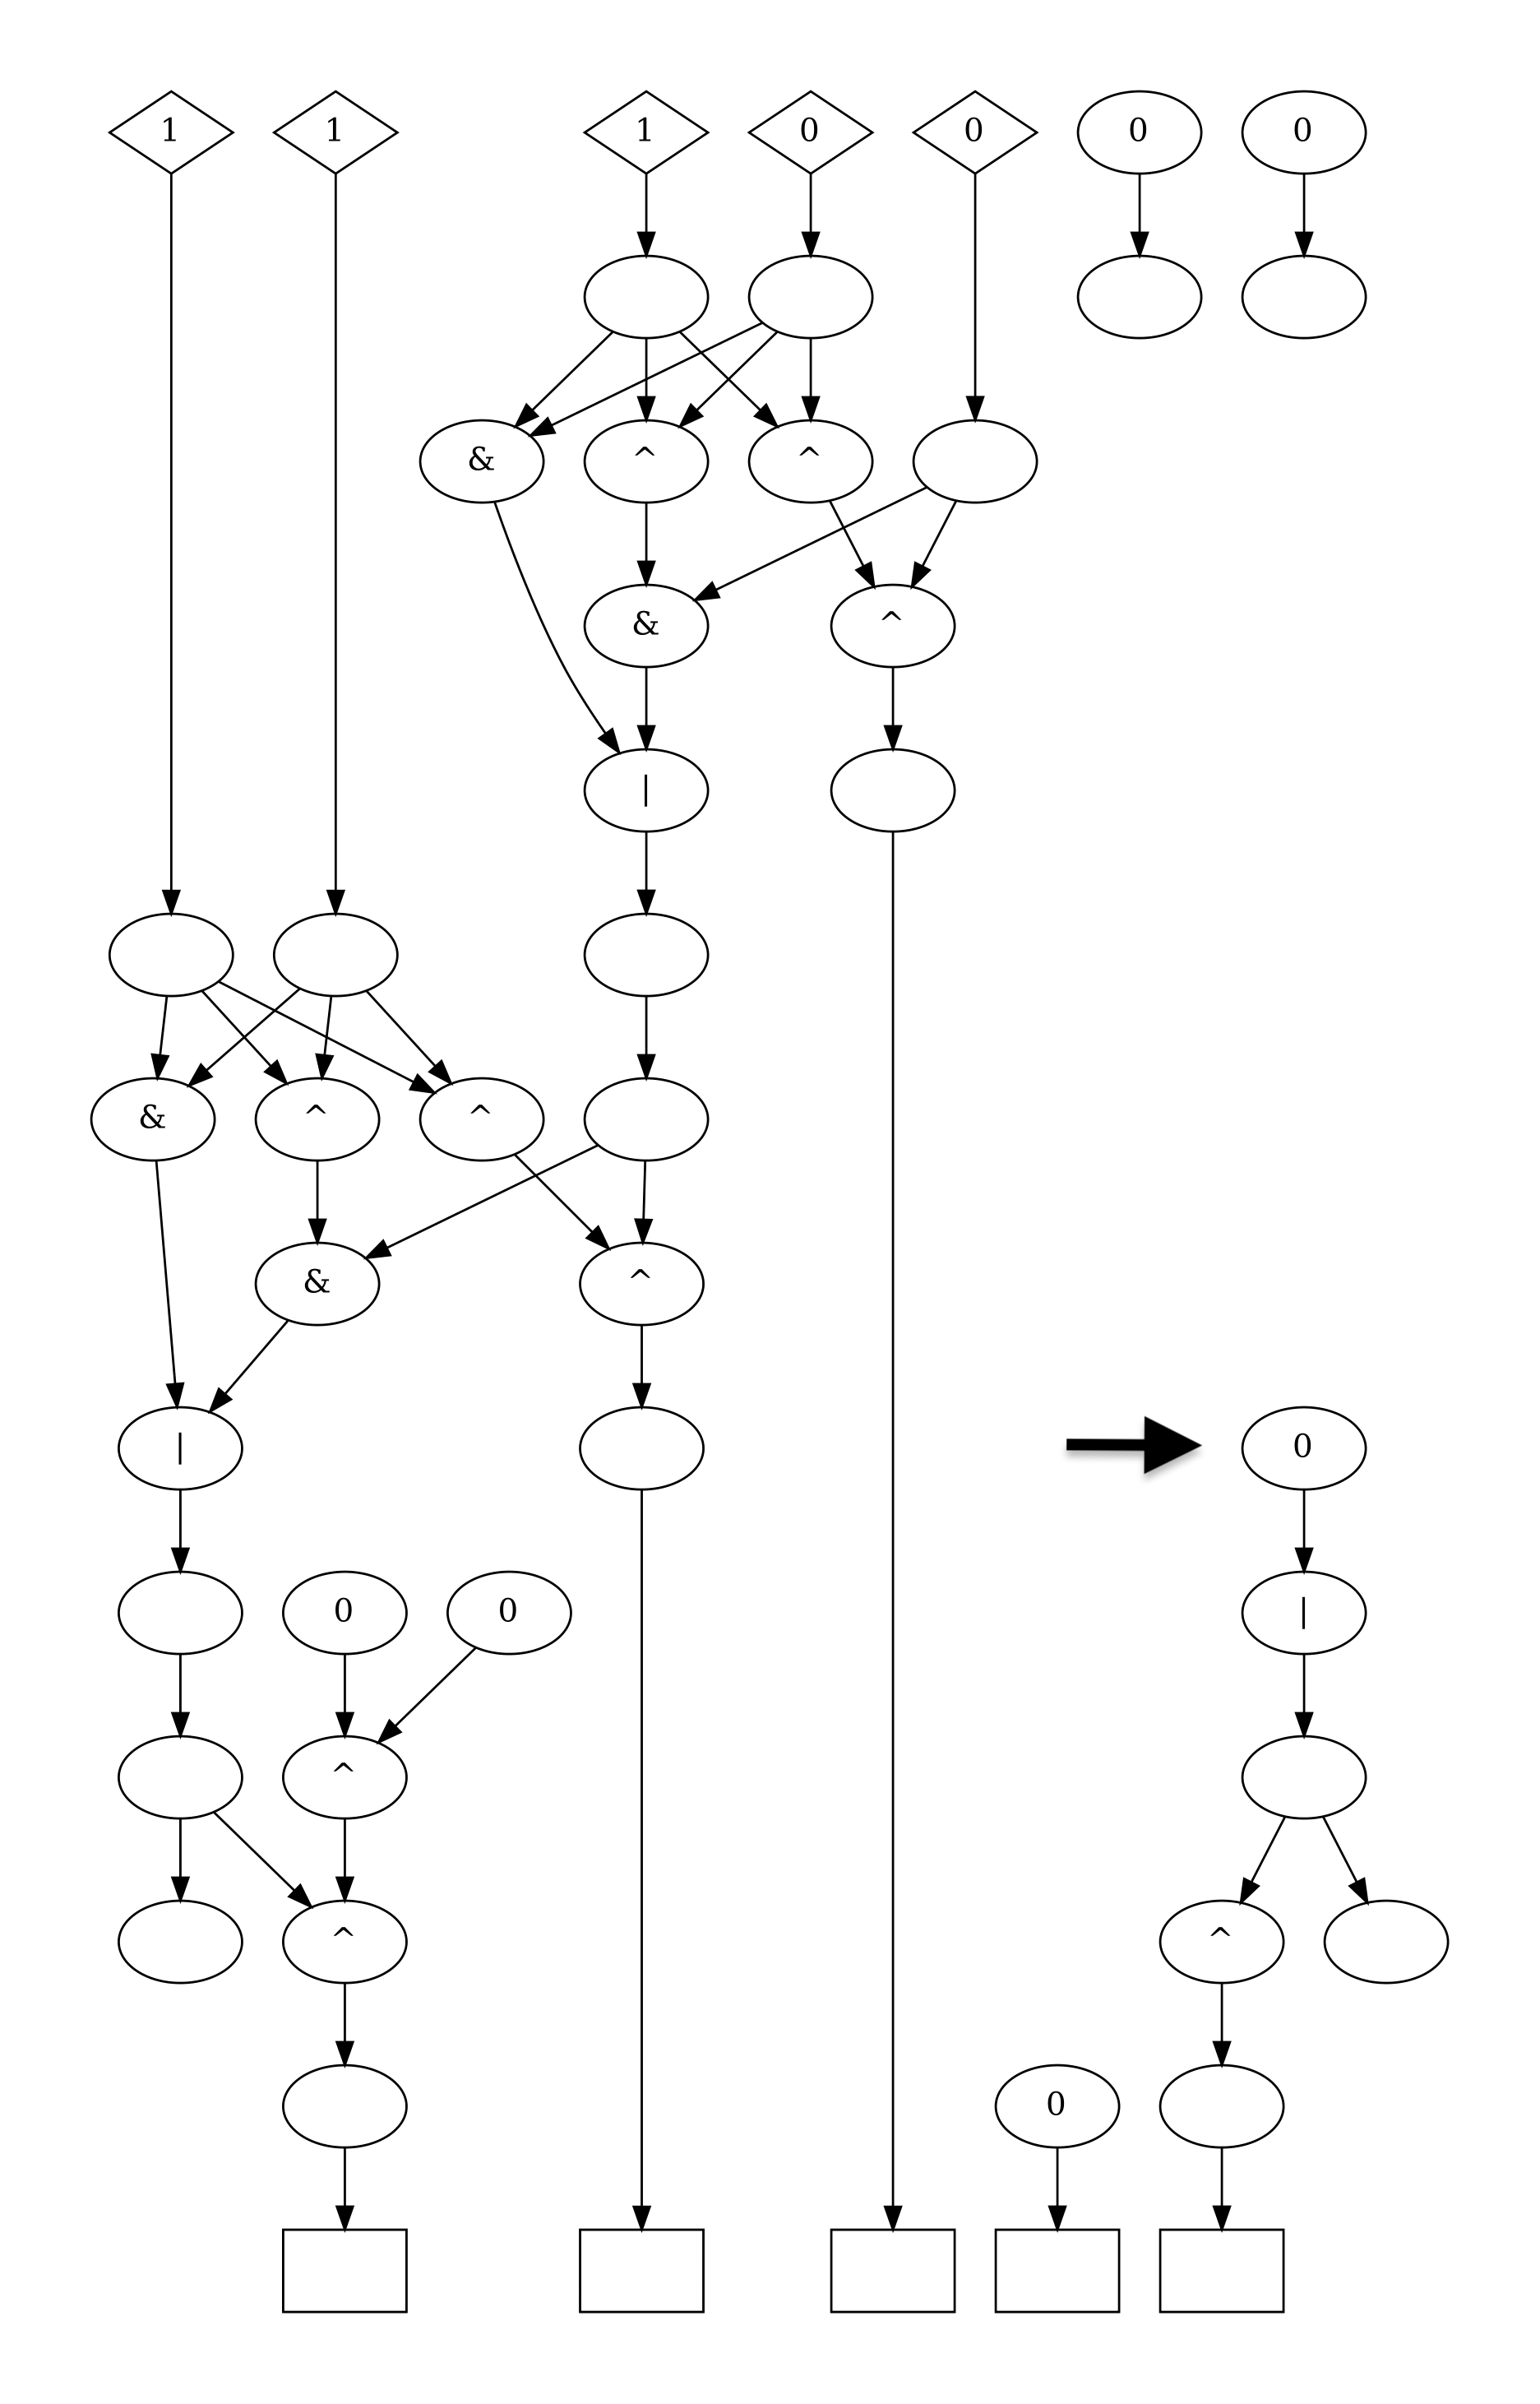
\includegraphics[width=0.9\textwidth]{figures/half_adder/debug_evualte_16-1.png}
        \end{minipage}
        \begin{minipage}{0.49\textwidth}
            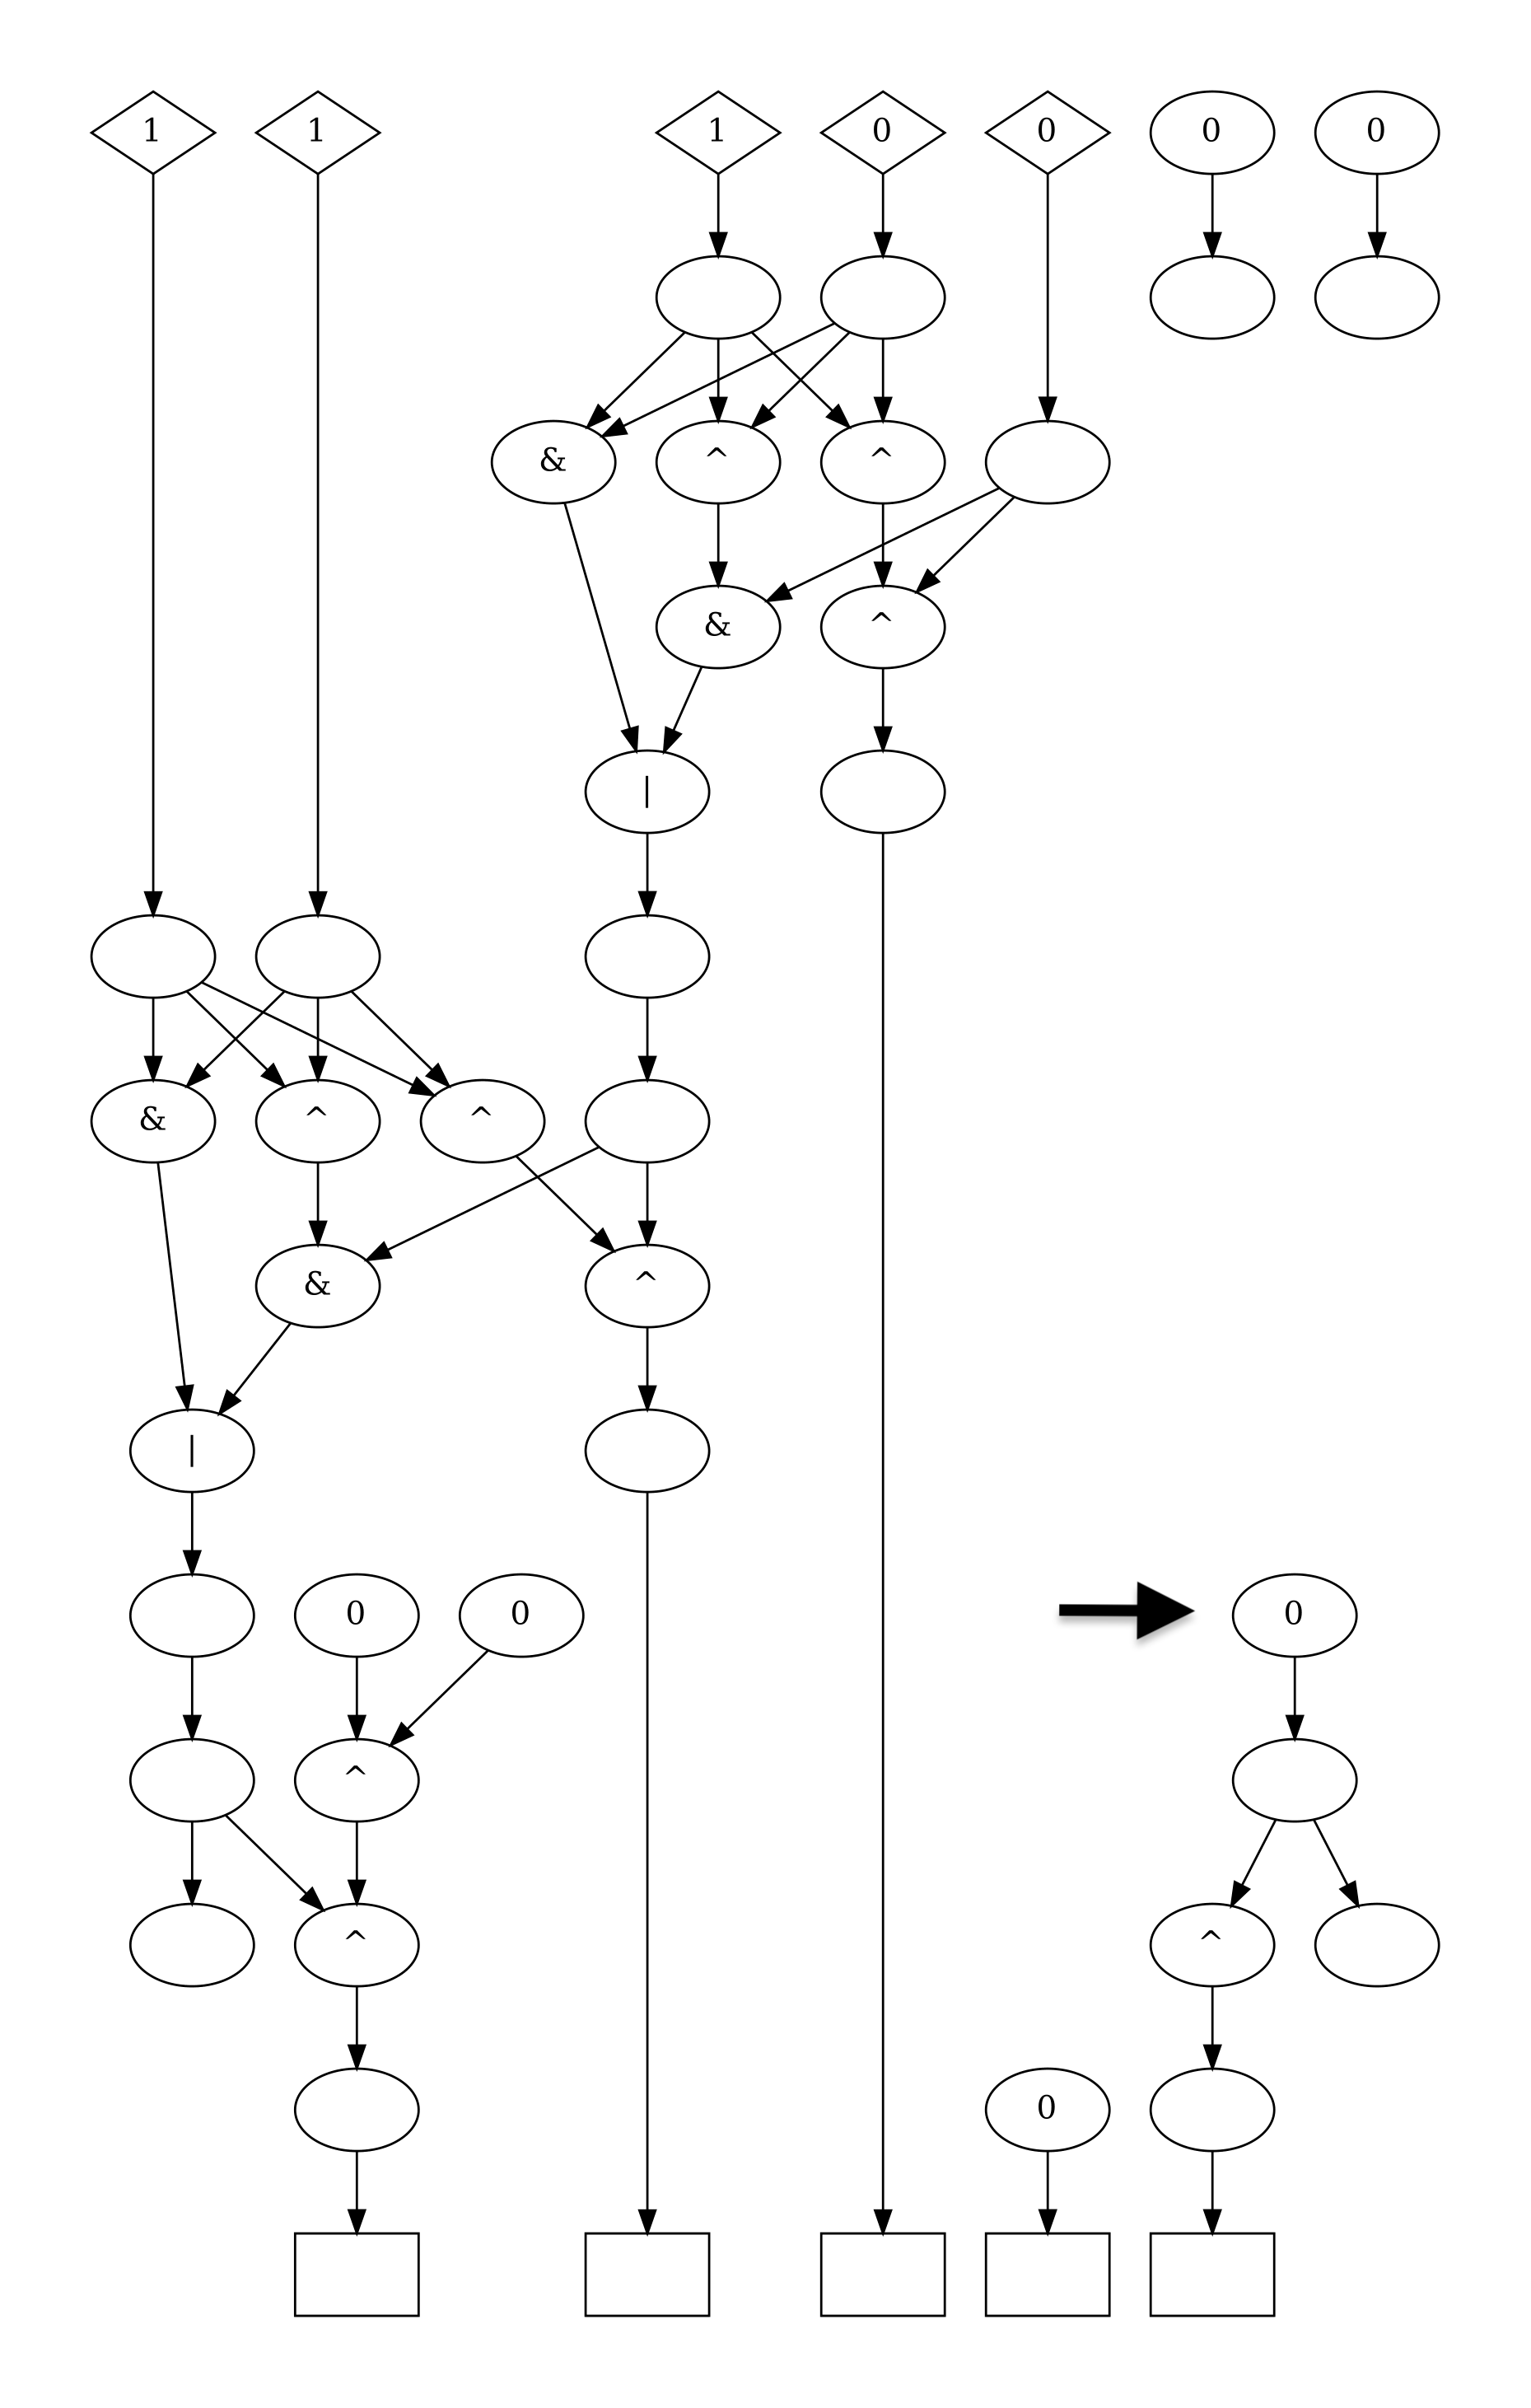
\includegraphics[width=0.9\textwidth]{figures/half_adder/debug_evualte_17-1.png}
        \end{minipage}
    \caption{Comparaison de l'état de half-adder avant et apres d'une application d'une transformation intermédiaire ($0 | 0 = 0$)}
    \label{fig:half-adder-comparaison}
\end{figure}
\begin{figure}[H]
    \centering
    \begin{minipage}{0.49\textwidth}
        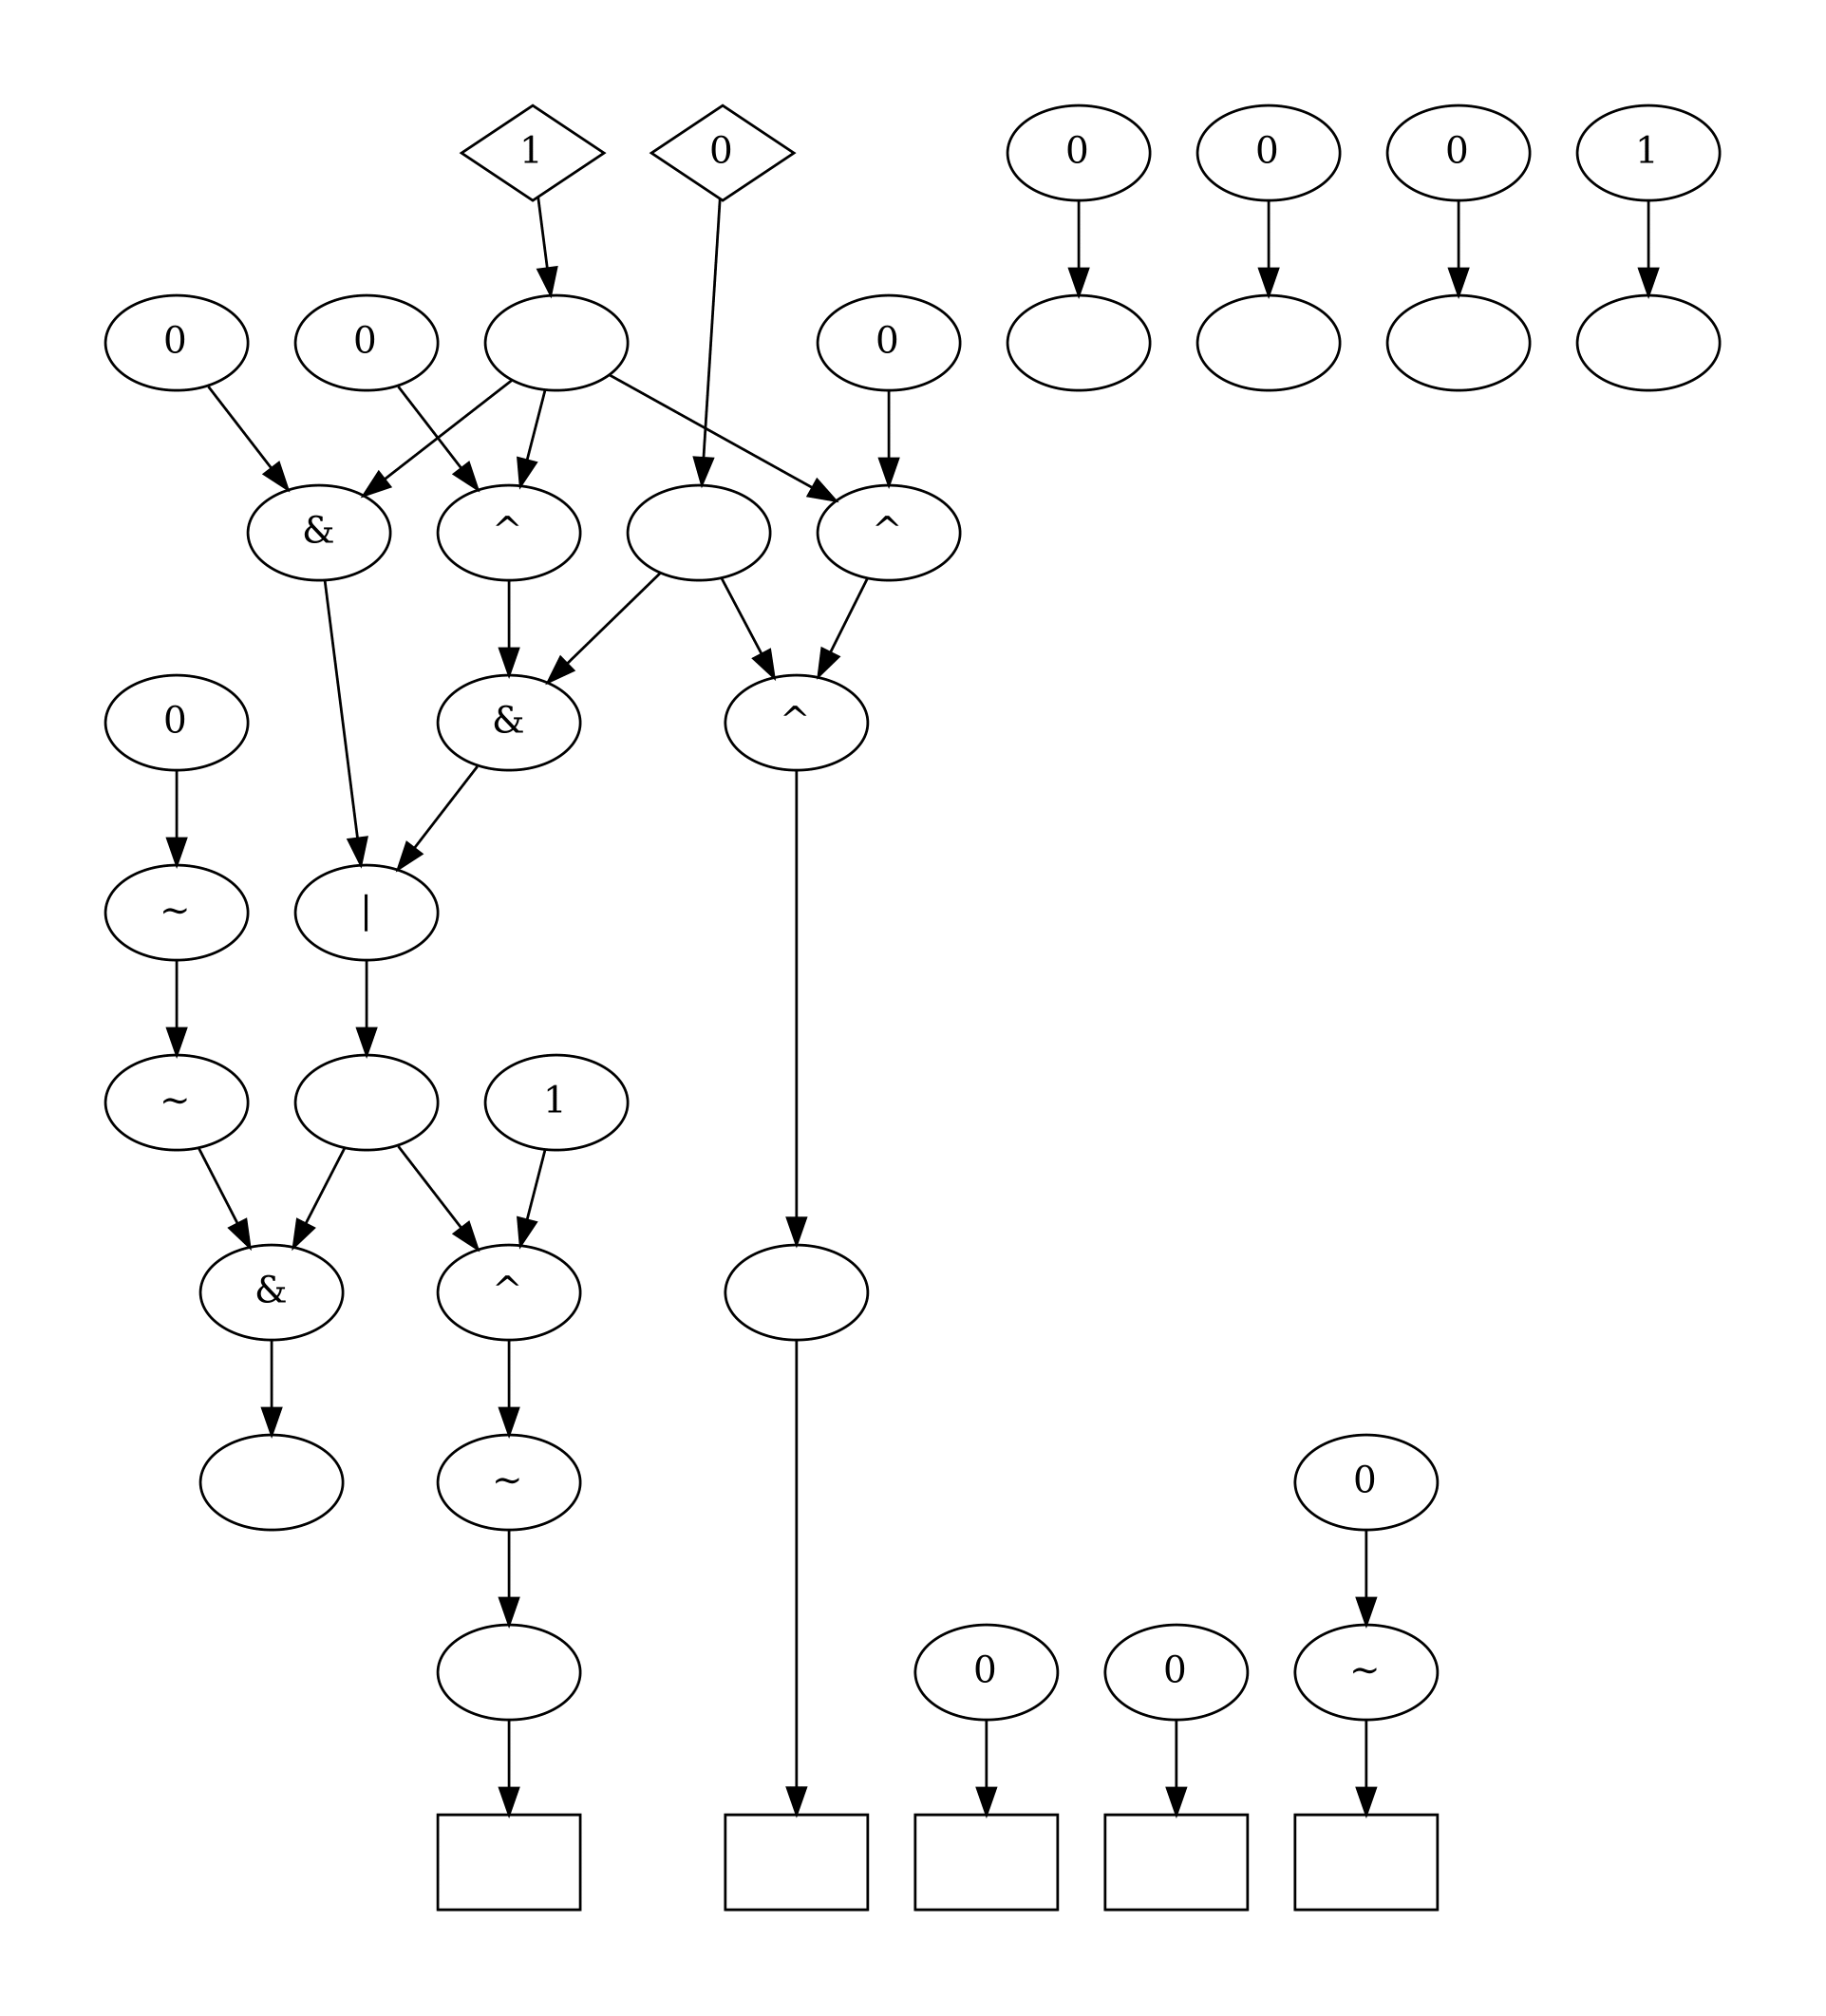
\includegraphics[width=0.9\textwidth]{figures/half_adder/debug_evualte_35-1.png}
    \end{minipage}
    \begin{minipage}{0.49\textwidth}
        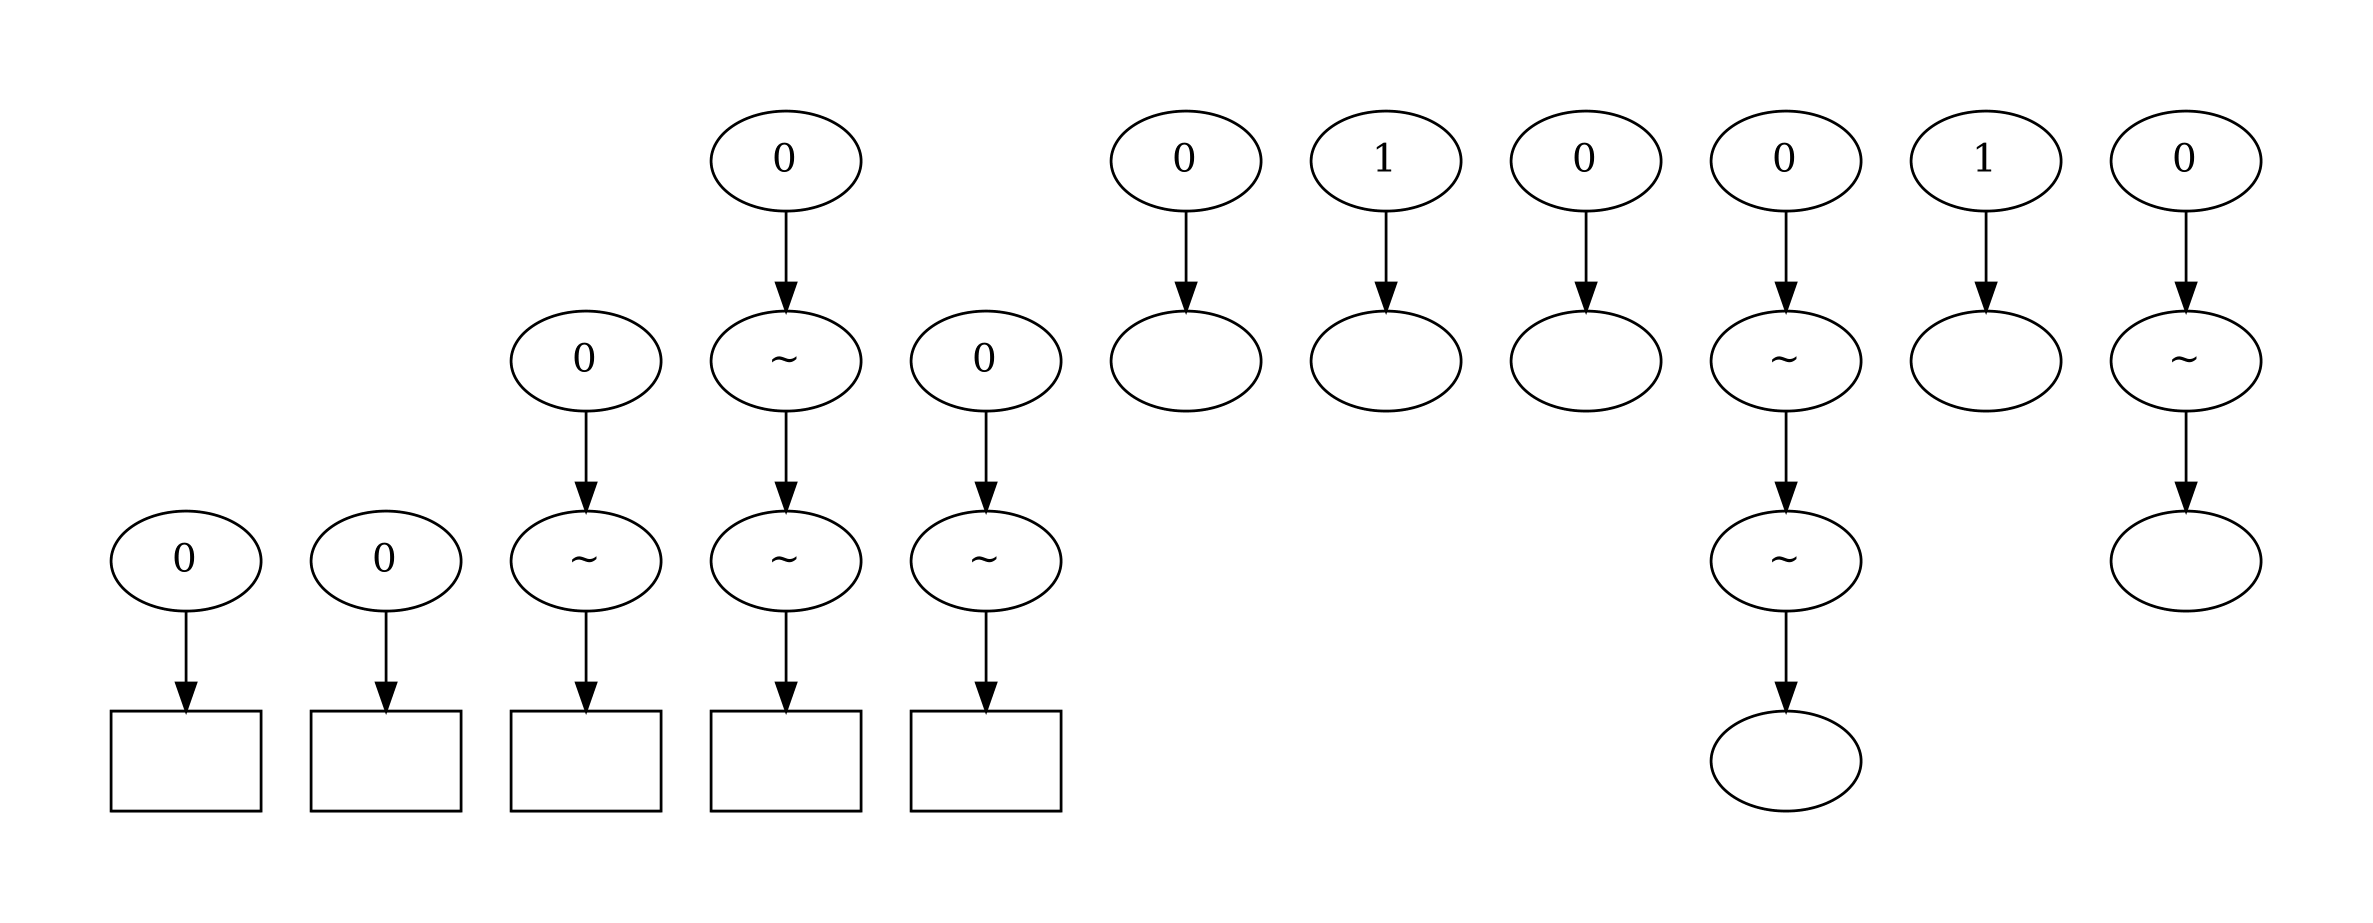
\includegraphics[width=0.9\textwidth]{figures/half_adder/debug_evualte_51-1.png}
    \end{minipage}
    \caption{Les étapes avant la finalisation de l'évaluation de half-adder}
    \label{fig:etapes-avant-la-finalisation-de-l-evaluation-de-half-adder}
\end{figure}

\begin{figure}[H]
    \centering
    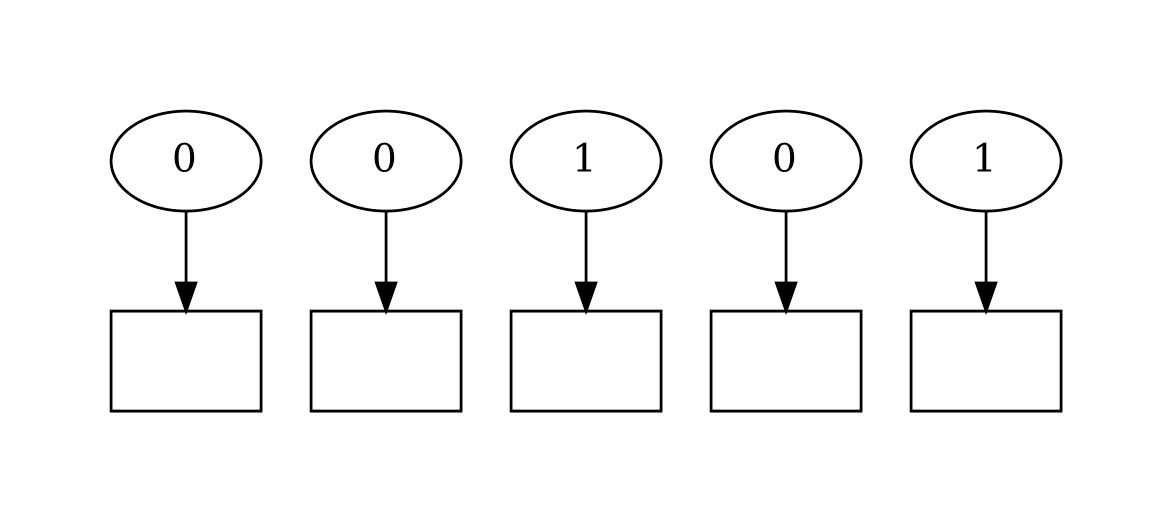
\includegraphics[width=0.5\textwidth]{figures/half_adder/debug_evualte_62-1.png}
    \caption{L'état de \textit{half-adder} après l'évaluation complète}
    \label{fig:etat-de-half-adder-apres-l-evaluation-complete}
\end{figure}

\subsection{Les figures de l'encodeur et décodeur}
\begin{figure}[H]
    \centering
    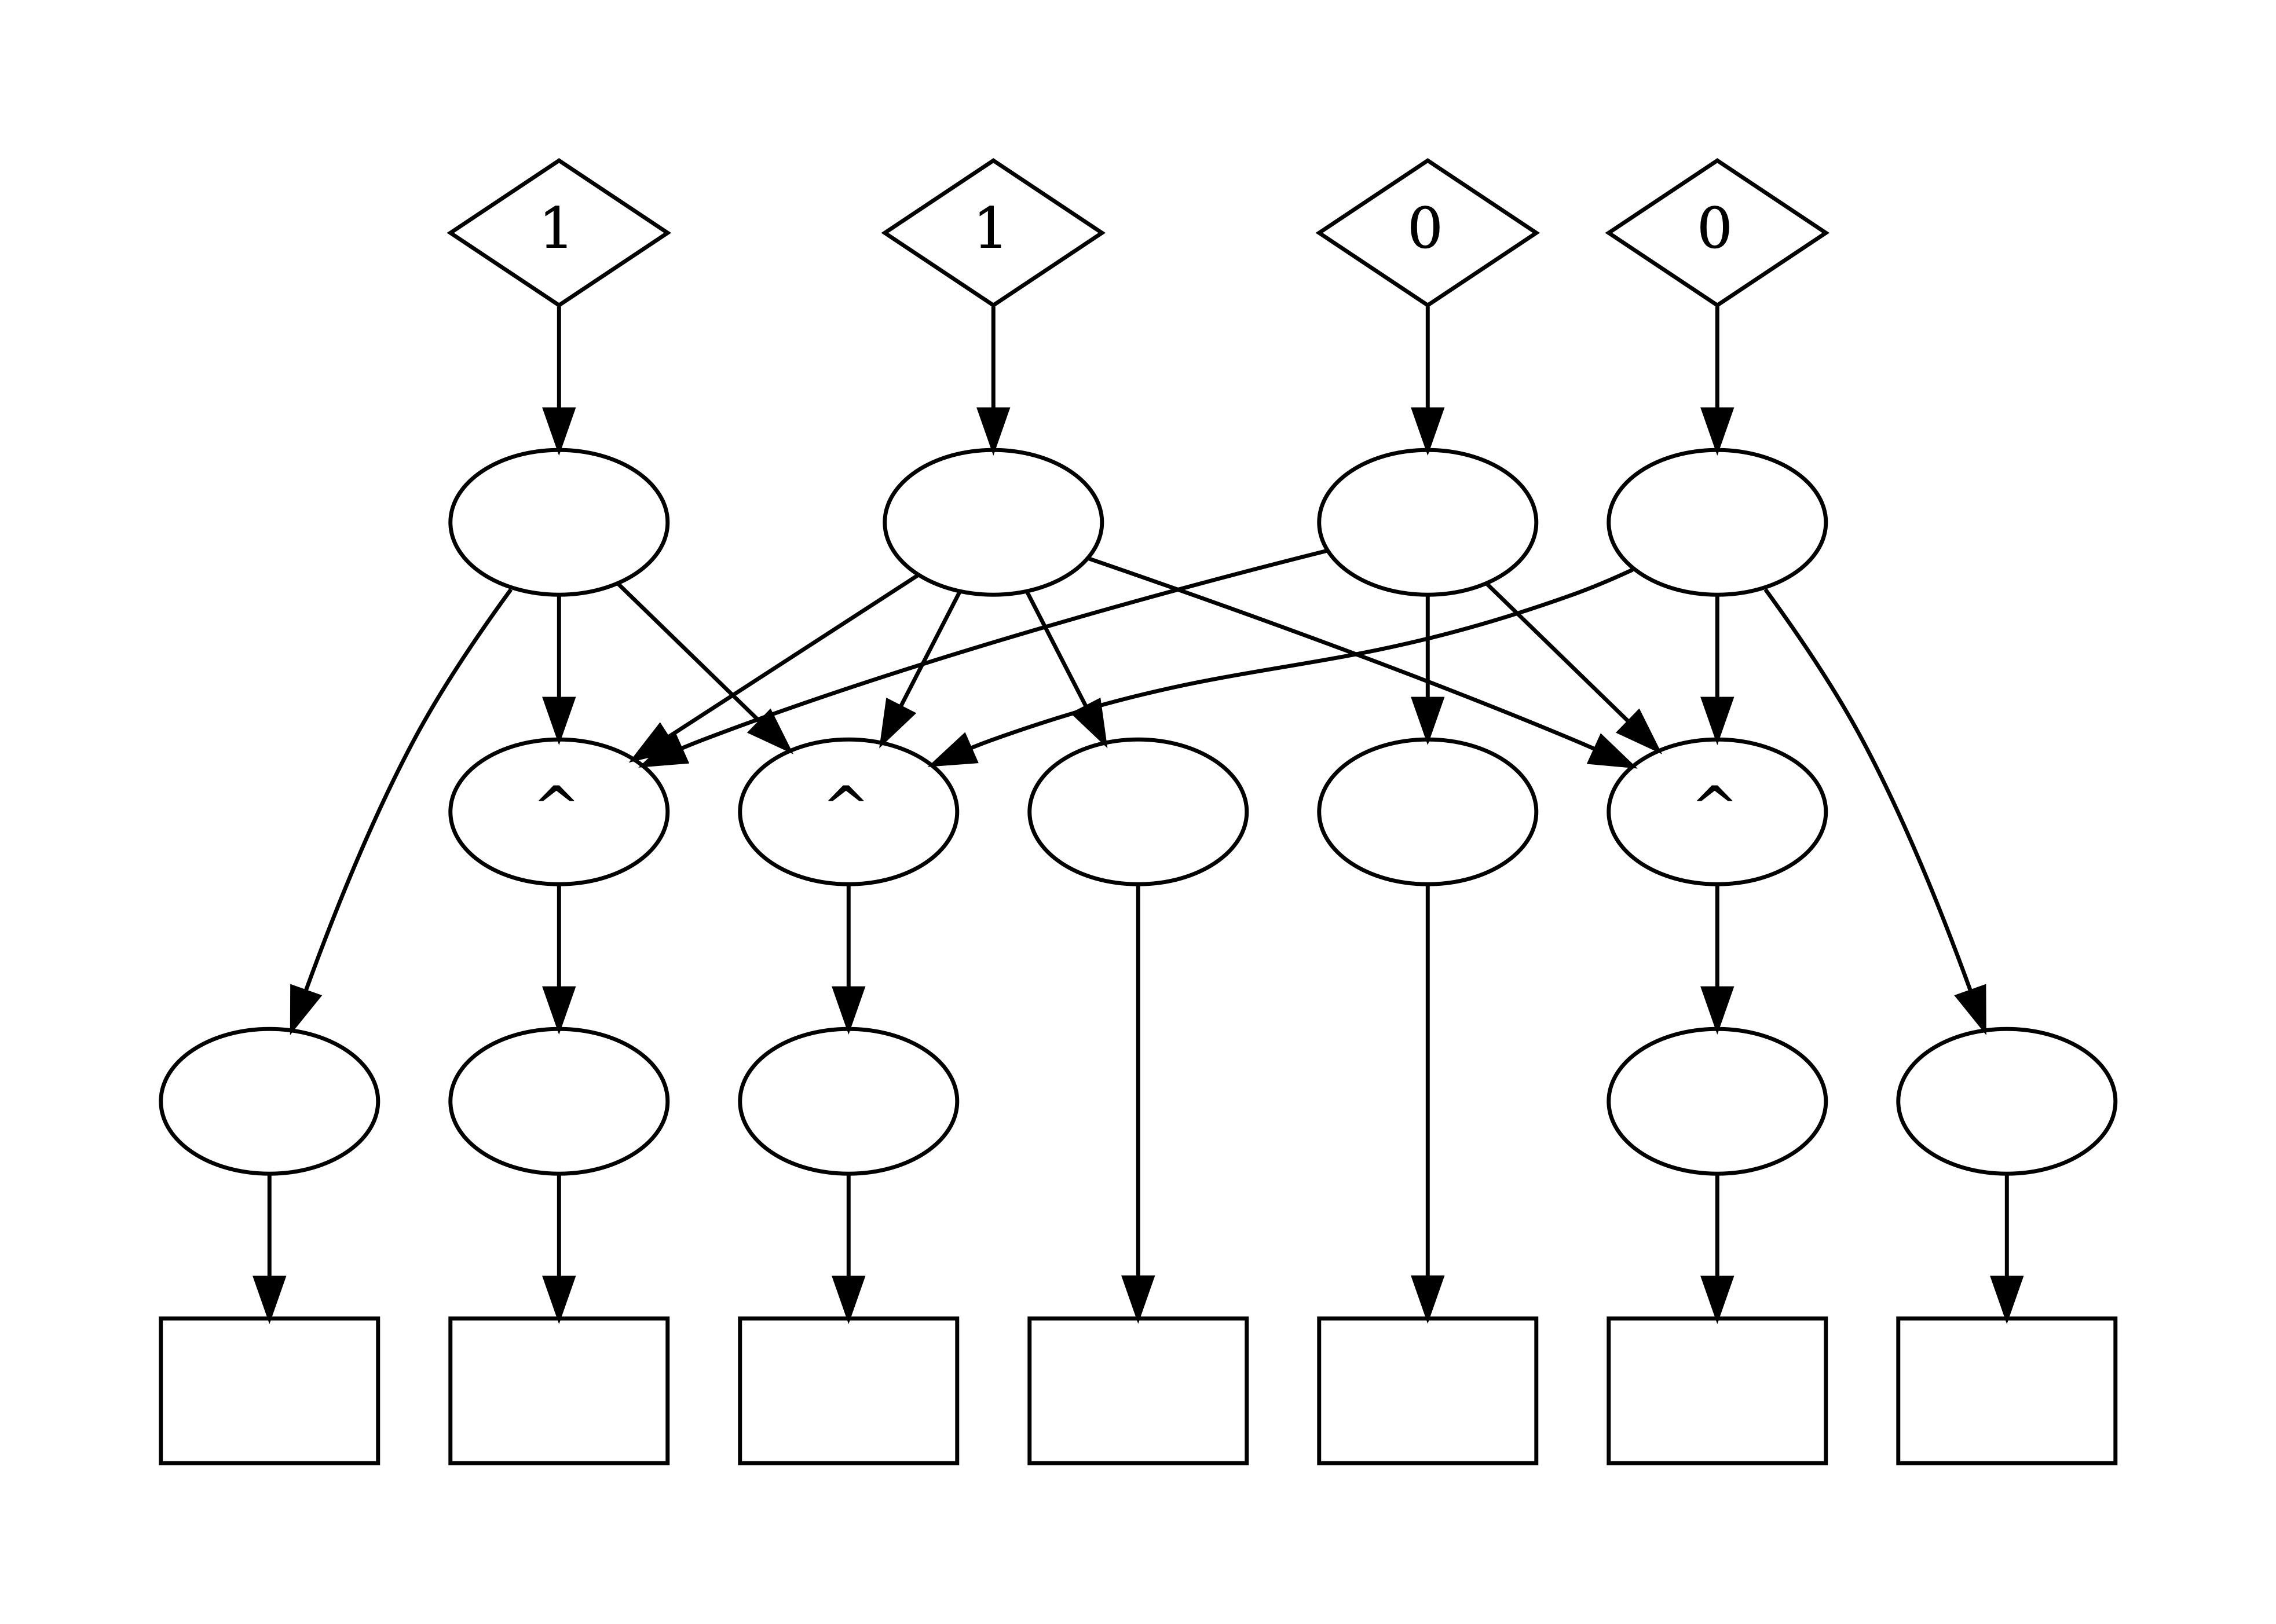
\includegraphics[width=0.8\textwidth]{figures/no_error/encoder.png}
    \caption{L'encodeur}
    \label{fig:encoder-no-error}
\end{figure}

\begin{figure}[H]
    \centering
    \includegraphics[width=0.8\textwidth]{figures/no_error/decoder.png}
    \caption{Le décodeur}
    \label{fig:decoder-no-error}
\end{figure}

\begin{figure}[H]
    \centering
    \includegraphics[width=0.8\textwidth]{figures/no_error/comp.png}
    \caption{La composition de l'encodeur et déodeur}
    \label{fig:compos-enc-dec-no-error}
\end{figure}

\begin{figure}[H]
    \centering
    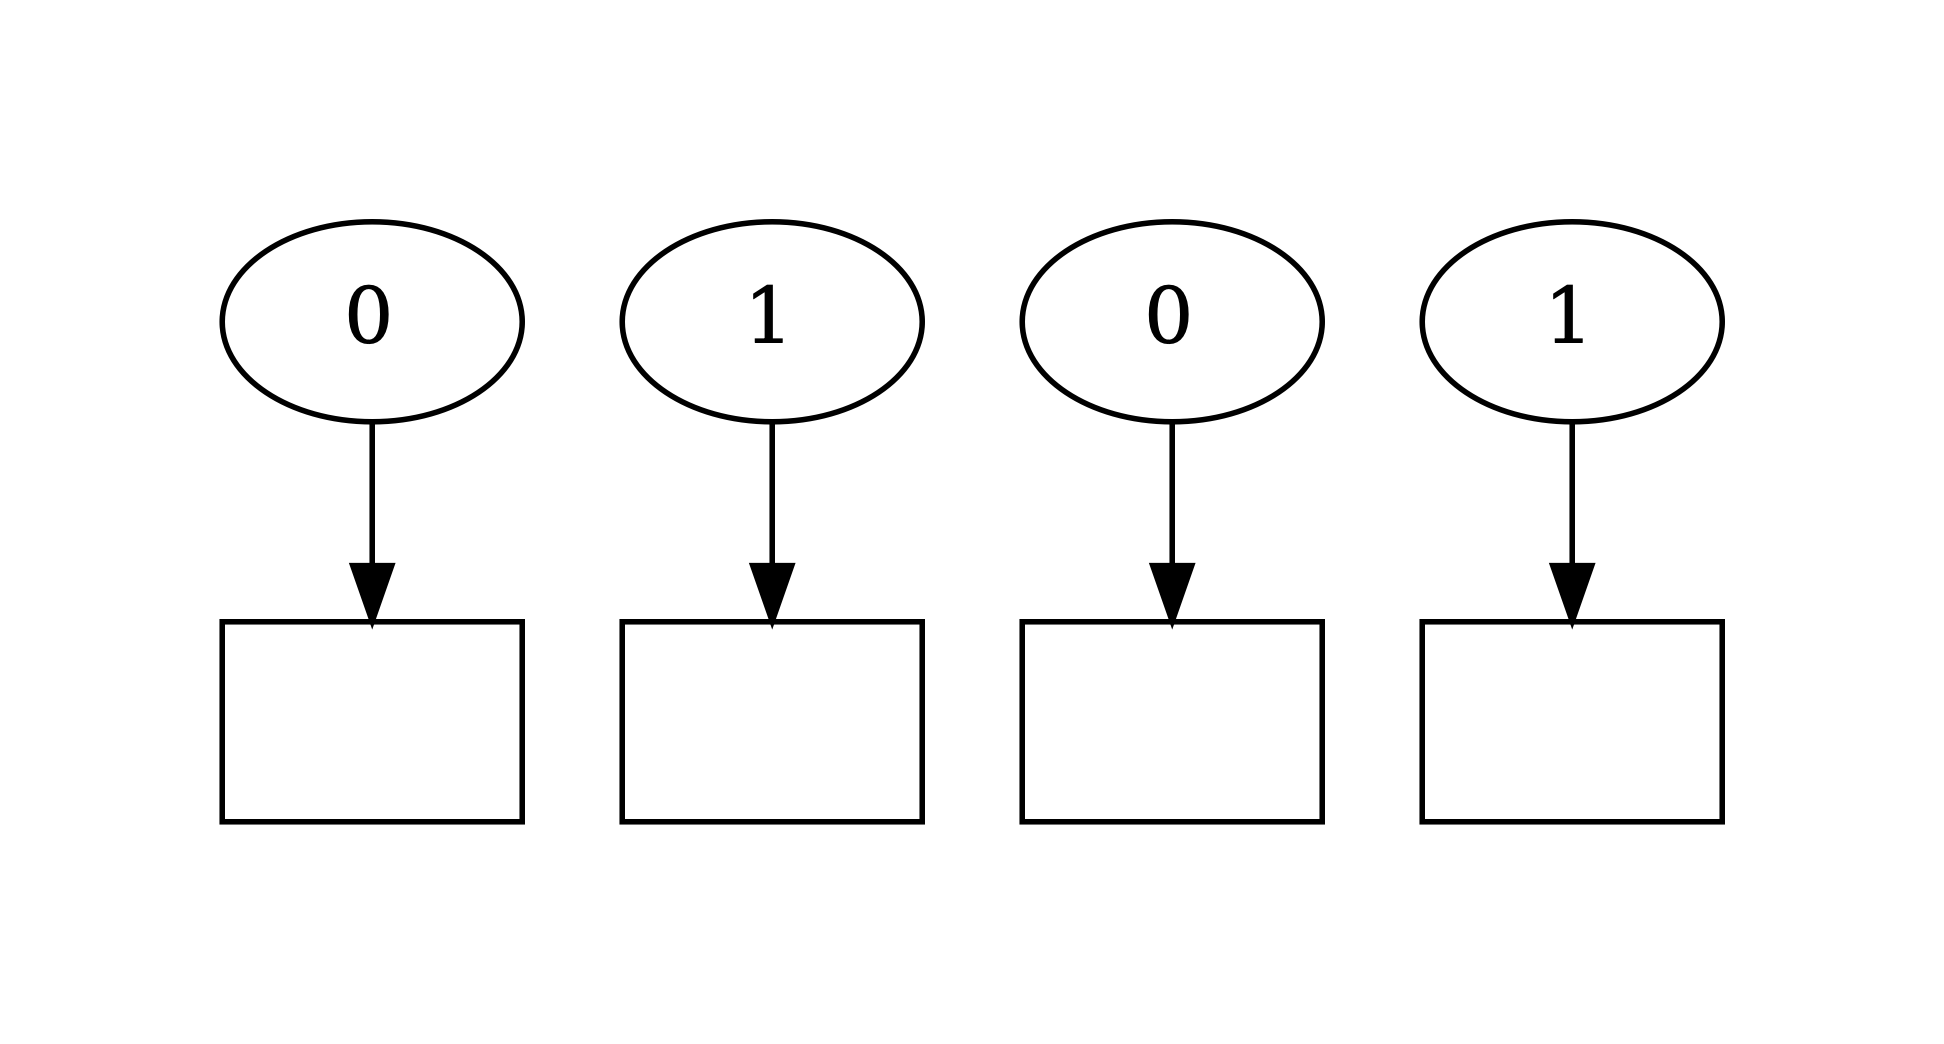
\includegraphics[width=0.8\textwidth]{figures/no_error/encoder_decoder_compose.png}
    \caption{L'identité après l'évaluation de la composition de l'encodeur et le décodeur}
    \label{fig:enc-dec-identity}
\end{figure}

\begin{figure}[H]
    \centering
    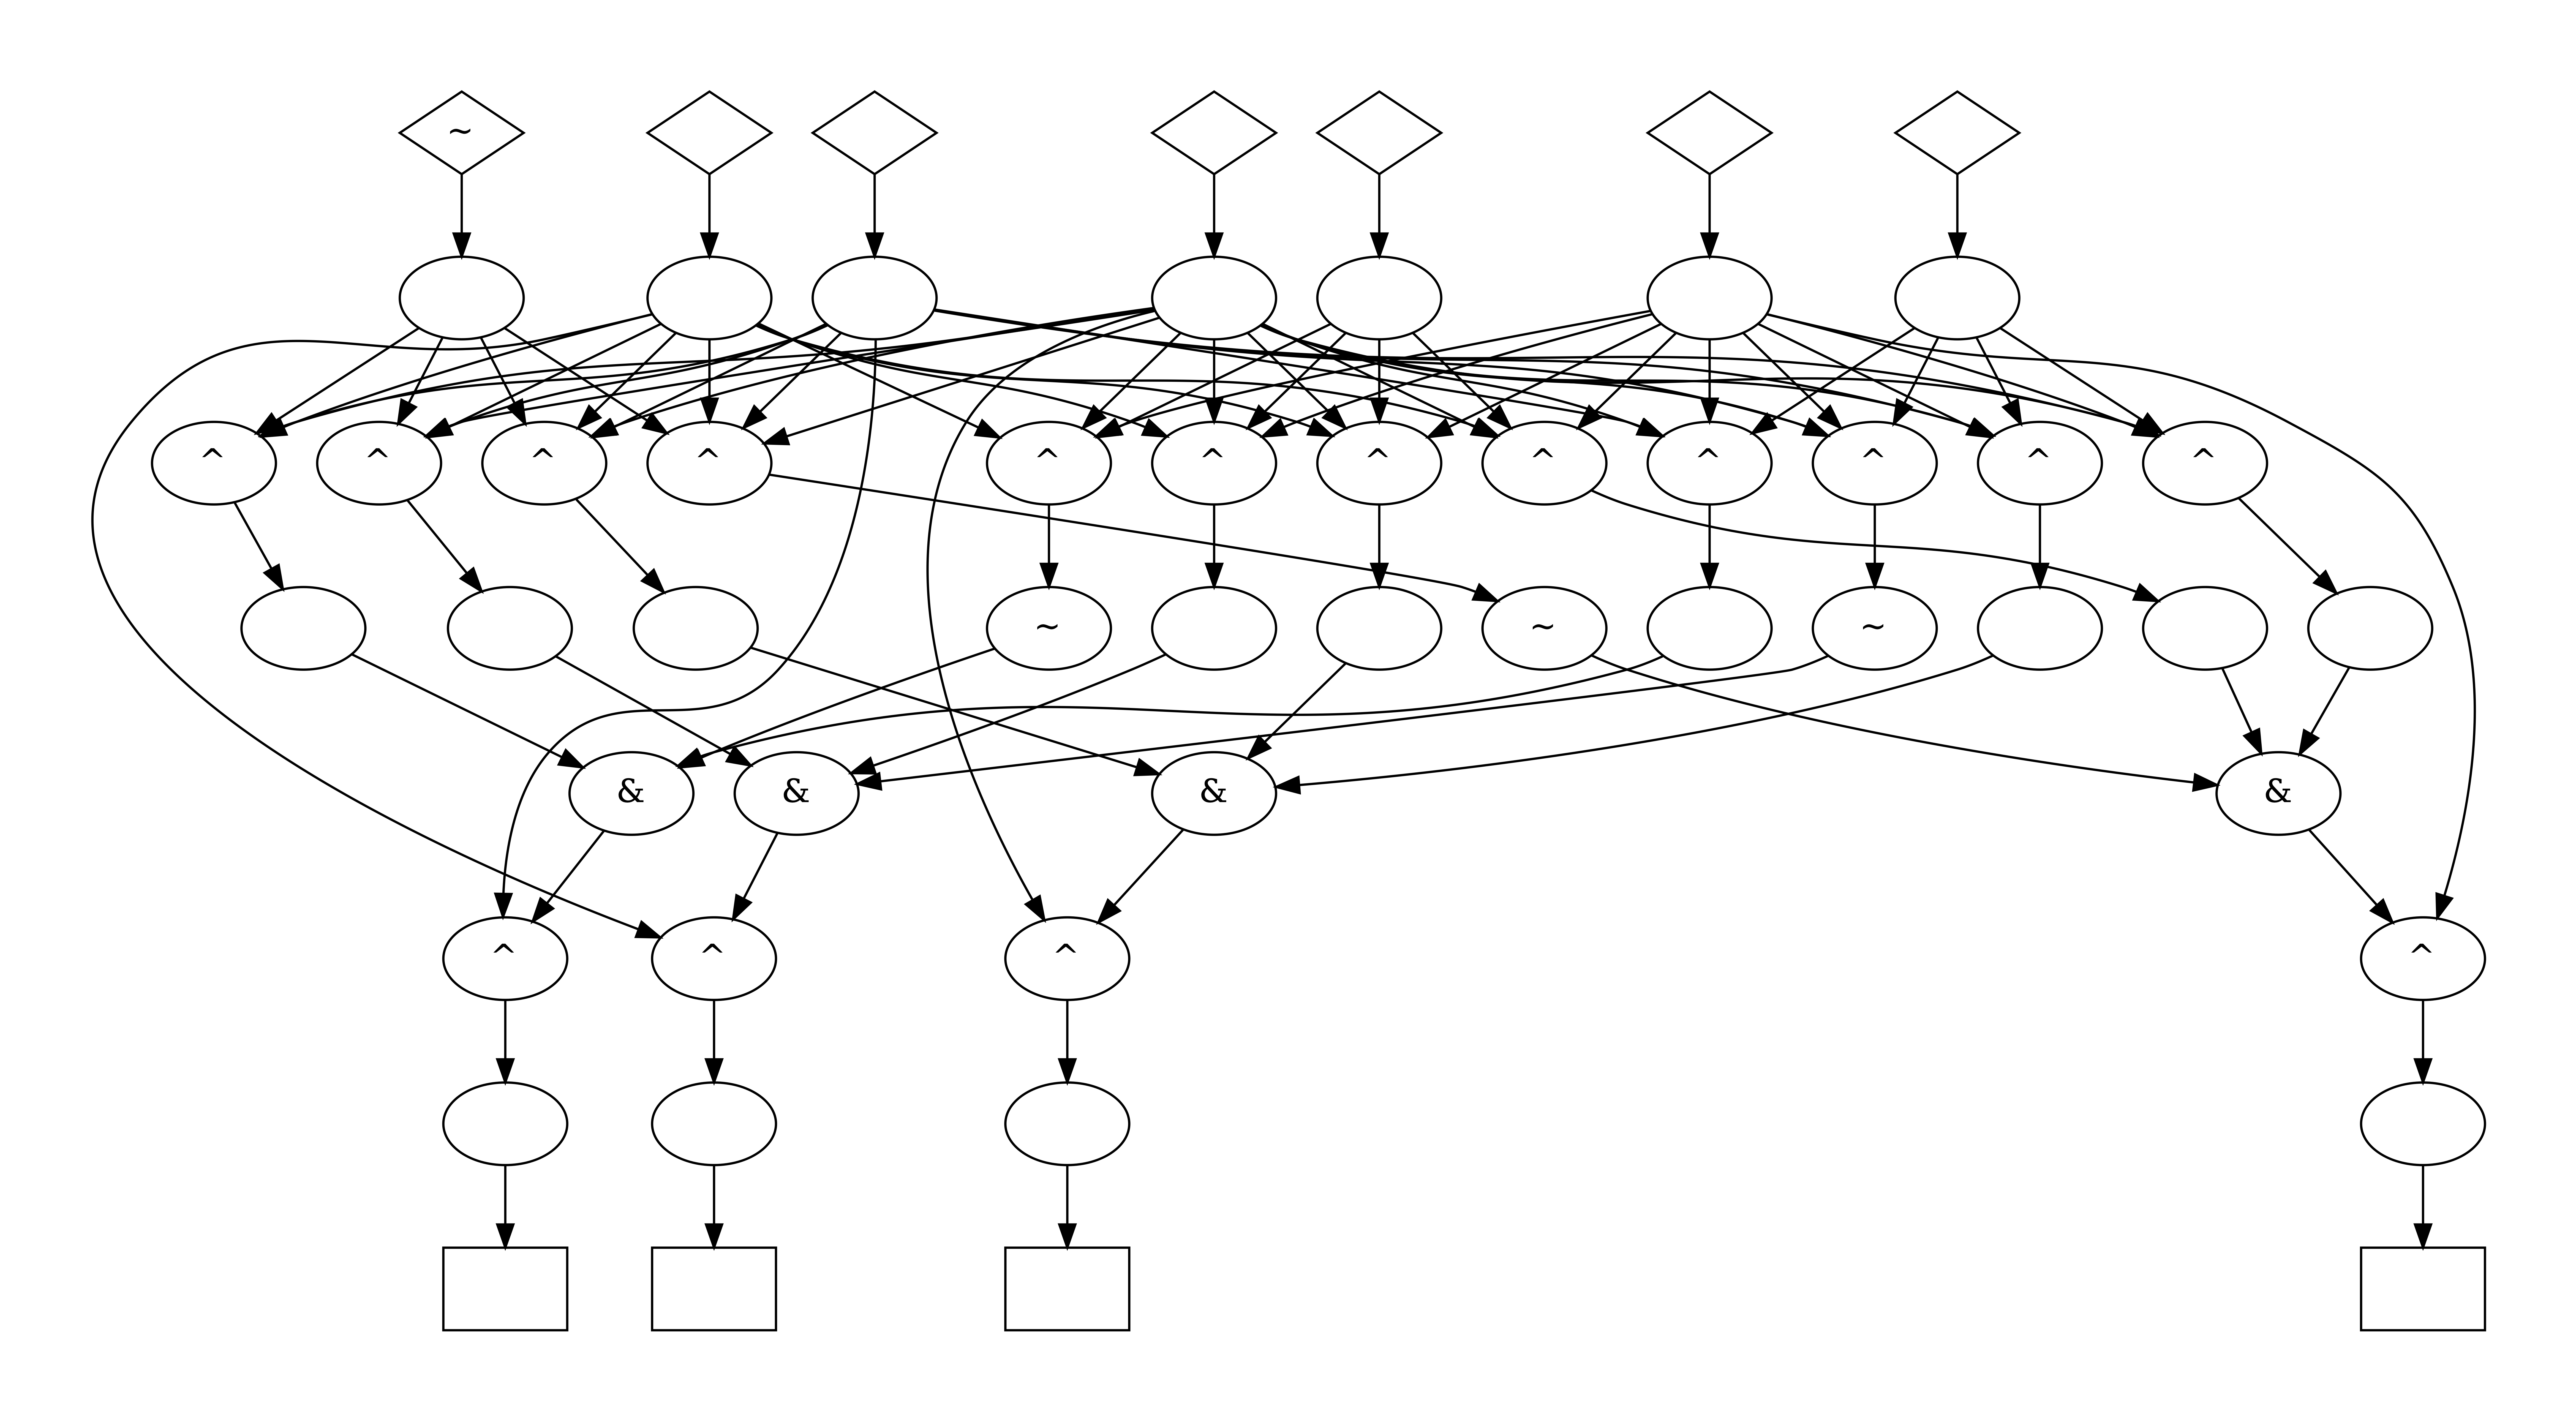
\includegraphics[width=0.8\textwidth]{figures/one_error/dec_g.png}
    \caption{Le décodeur avec une erreur (une porte non)}
    \label{fig:decoder-with-one-error}
\end{figure}

\begin{figure}[H]
    \centering
    \includegraphics[width=0.8\textwidth]{figures/one_error/comp.png}
    \caption{La composition de l'encodeur et du décodeur avec une erreur (une porte non)}
    \label{fig:encode-decode-compose-one-error}
\end{figure}

\begin{figure}[H]
    \centering
    \includegraphics[width=0.8\textwidth]{figures/two_errors/decoder.png}
    \caption{Le décodeur avec deux erreurs (voir deux portes non dans les inputs)}
    \label{fig:decoder-two-errors}
\end{figure}

\begin{figure}[H]
    \centering
    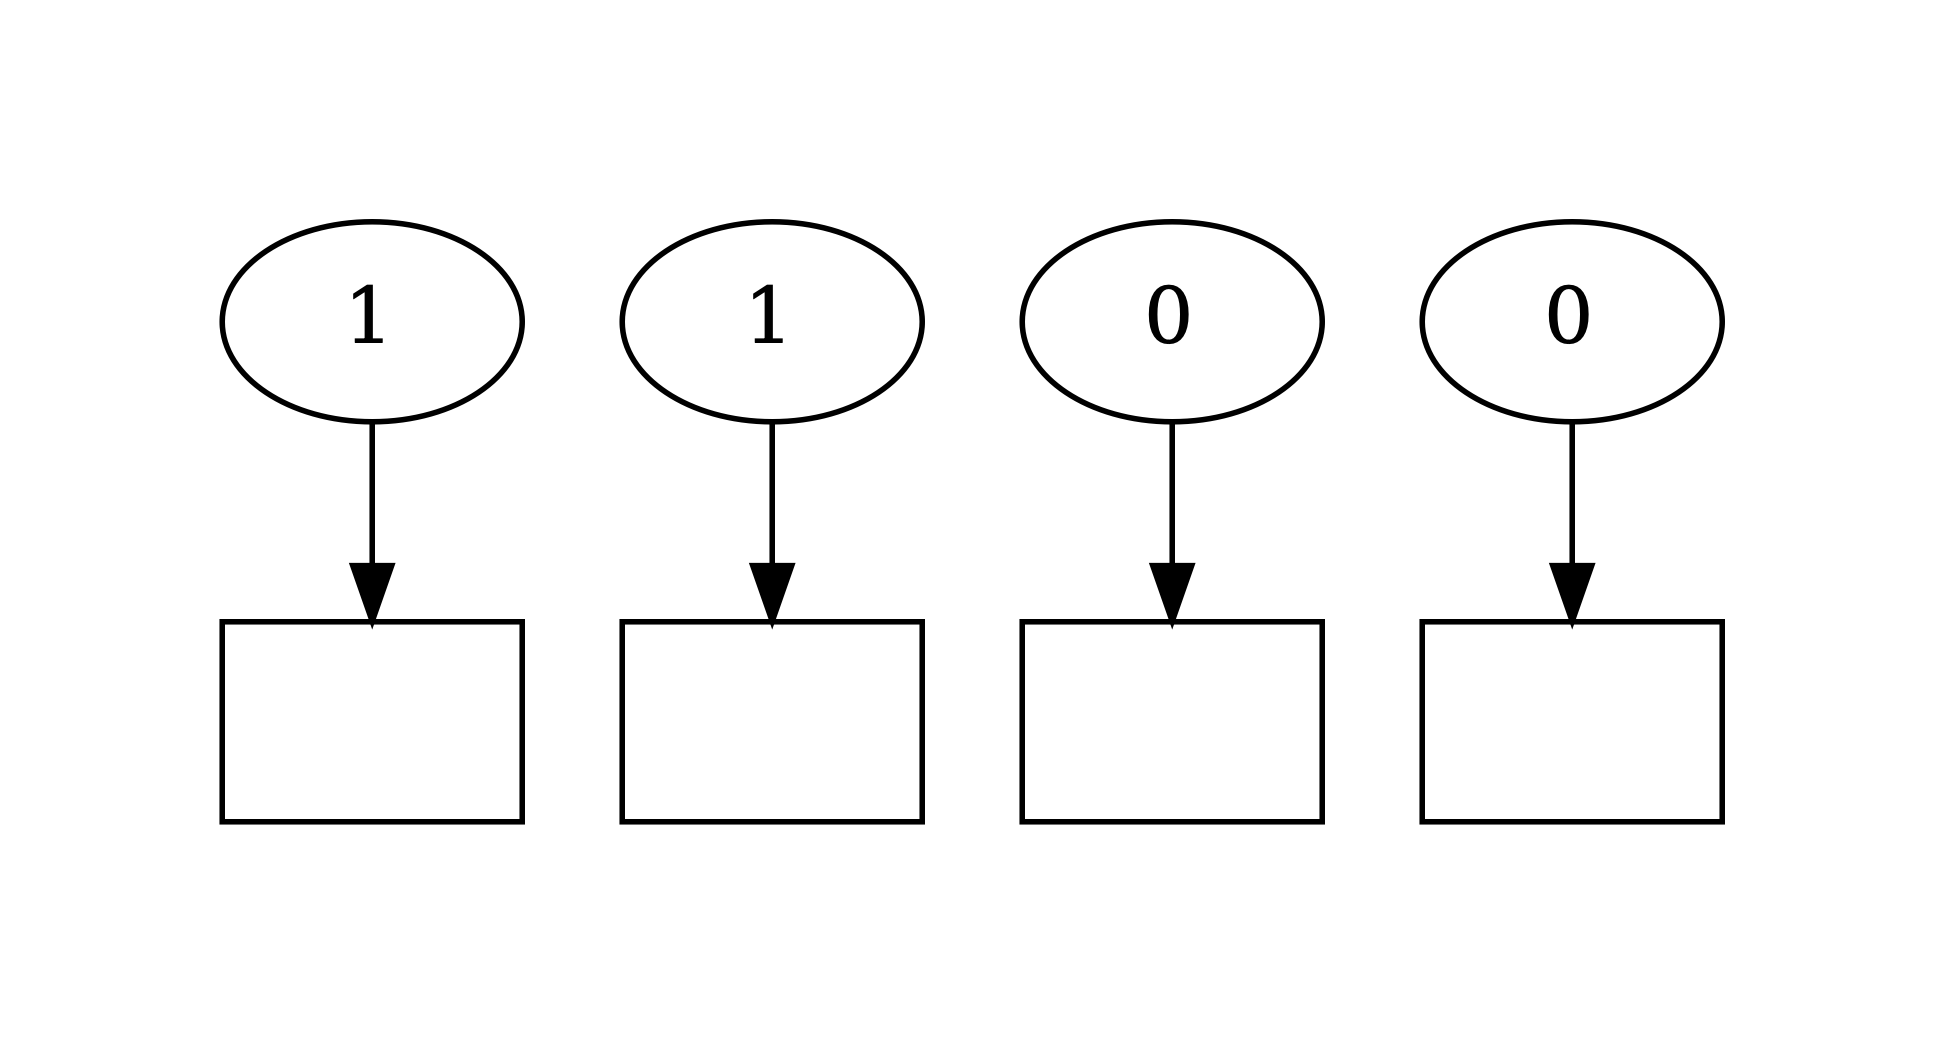
\includegraphics[width=0.8\textwidth]{figures/two_errors/encoder_decoder_compose.png}
    \caption{L'identité avec les bits changés qui ne correspondent pas aux bits initiales}
    \label{fig:identity-two-errors}
\end{figure}

\listoffigures
\end{document}
